\documentclass[12pt,a4paper]{report}

\usepackage[a4paper,margin=2.5cm]{geometry}
\usepackage[T1]{fontenc}
\usepackage{lmodern}
\usepackage[english]{babel}
\usepackage{setspace}
\usepackage{amsmath,amssymb}
\usepackage{booktabs}
\usepackage{graphicx}
\usepackage{multirow}
\usepackage{array}
\usepackage{tabularx}
\usepackage{float}
\usepackage{xcolor}
\usepackage{tikz}
\usetikzlibrary{arrows.meta,positioning,fit,calc}
\usepackage[authoryear,round]{natbib}
\usepackage[hidelinks]{hyperref}

\onehalfspacing

\newcommand{\todo}[1]{\textcolor{red}{[TODO #1]}}
\newcommand{\sig}{$^{*}$}

\begin{document}

% Title page
\begin{titlepage}
\centering
\vspace*{1.5cm}
{\bfseries\large Kandy Innovation Centre,\par}
{\bfseries\large National Institute of Business Management.\par}
\vspace{2.5cm}
{\Large \bfseries UNDERGRADUATE RESEARCH THESIS\par}
\vspace{2.5cm}
% Logos as in the literature review. Upload the two image files, then uncomment.
% \includegraphics[height=1.6cm]{nibm_logo.jpg}\hspace{2cm}\includegraphics[height=1.6cm]{kic_logo.jpeg}
\vspace{2.5cm}
{\large \bfseries Session-Persistent Test-Time Training for Language Models\par}
\vspace{0.4cm}
{\normalsize A Carried Fast Weight Transfers to Related Documents and Hurts Unrelated Ones\par}
\vspace{2cm}
{\normalsize M A S I Malimbada, \textsc{KIC-BSCCSAI-25.1-P-014}\par}
\vspace{0.6cm}
{\normalsize Supervisor, Prof. Roshan D. Yapa\par}
\vfill
{\large Kandy Innovation Centre,\par}
{\large National Institute of Business Management,\par}
{\large 1095, Kandy Colombo Road, Getambe.\par}
\end{titlepage}

\pagenumbering{roman}

\chapter*{Abstract}
\addcontentsline{toc}{chapter}{Abstract}

Test-time training (TTT) lets a language model update part of its weights while it reads, but existing designs discard that adaptation at every document boundary. This thesis asks whether the adapted fast weights can be carried into the next document, how much that carry contributes (Q1), and which domains benefit most (Q2). The main finding is that a trained, gated fast-weight carry transfers to related documents and hurts unrelated ones. On 200 Wikipedia articles, a carry built from an article that the target mentions lowers the target's perplexity by 0.085, one built from an unrelated article by 0.051, and one built from text of another source raises it by 0.067, with every step of this gradient significant and replicated with a second training seed. Against dynamic evaluation tuned for the same transfer, the carry transfers about 0.3 percent more to related and to unrelated articles of the same source, using forward passes only, while dynamic evaluation adapts more strongly to a document's own text. The carry does not accumulate. Re-reading a document ten times helps no more than reading it twice.

We reach this design through a diagnosis. We add In-Place TTT layers to the MLP down-projections of Qwen3-0.6B, train them with a Hebbian and a chunked delta update rule, and compare them against a LoRA-only model trained with identical data, schedule and learning rate, using paired evaluation regimes on 106 held-out documents from six domains. A naive carry contributes nothing measurable across documents, for both rules and at every checkpoint. The read-time norm clip that keeps the fast weights stable is active on every measurement by a factor of at least 255, so only the direction of the carried state reaches the output, and removing the clip makes training collapse or switches the fast weights off. The redesign gives the carry its own clipped path with its own gate and a zero-initialised scale, trains it through the boundary between slices, and starts the main gate nearly closed. An ablation shows that the first two changes are both needed and work together.

Within a document, the redesigned carry lowers perplexity on later slices by 0.06 to 0.14 through 600 training steps, against 0.002 to 0.014 for the original design, and the model leads the matched LoRA baseline by 0.234 perplexity, more than either original rule. Placing the previous text directly in attention is far stronger, and the carry recovers about four percent of its gain, so its use is where attention cannot reach. Most of a TTT model's lead over the matched baseline is the extra trainable capacity of the down-projection. For Q2, the within-document gain differs across domains but is not predicted by how hard a domain is for the base model.

\tableofcontents
\listoffigures
\listoftables

\clearpage
\pagenumbering{arabic}

% ======================================================================
\chapter{Introduction}
\label{ch-intro}

\section{Background}

A trained large language model answers every input with the same parameters. This makes inference efficient, but it also means the model cannot specialise to the context in which it is being used. Test-time training (TTT) relaxes this restriction by updating part of the model on the input it is currently reading, using a self-supervised objective that needs no labels \citep{sun2020ttt}. Applied to language models, TTT has been used to build sequence layers whose hidden state is itself a small model trained online \citep{sun2025learning}, long-term memory modules placed beside attention \citep{behrouz2025titans}, and most recently In-Place TTT \citep{feng2026inplace}, which turns the MLP down-projection of an existing transformer into a fast weight that adapts while the model reads.

\section{Research problem and gap}

Every one of these methods resets its adapted state at the end of each document. In-Place TTT does so deliberately, to prevent information leaking between unrelated inputs, and leaves the question of carrying the fast weights forward open \citep{feng2026inplace}. Related work approaches persistence from other directions. Some methods meta-learn a test-time initialisation or update weights over one long context \citep{tandon2025endtoend,bansal2025letsnot,wang2026learning}, and others carry cached activations or memory tokens across segments of a single stream \citep{dai2019transformerxl,bulatov2022rmt}. None carries a feed-forward fast weight across independently bounded documents. If such a carry worked, a model could keep improving on a user, a codebase or a domain without any gradient update to its slow weights, which is a form of continual learning at inference time.

\section{Research questions}

This thesis addresses two research questions, as stated in the research proposal.
\begin{description}
  \item[Q1.] How much does carry, the information retained from the previous session, contribute to language model improvement?
  \item[Q2.] What kind of domains perform best with session-persistent TTT?
\end{description}

\section{Objective}

The primary objective is to develop and empirically analyse a session-persistent test-time training method for pretrained language models. Following the proposal, the method exposes two logically independent components that can be measured separately, within-document adaptation without any persistence, and cross-document persistence of the fast weight.

\section{Contributions}

\begin{itemize}
  \item The finding that a trained, gated fast-weight carry transfers to related documents and hurts unrelated ones. Its benefit falls steadily with the relatedness of the earlier text, from a related article to an unrelated one, and turns to harm for text from another source. It transfers more than dynamic evaluation tuned for the same purpose, with forward passes only, it does not accumulate with repeated reading, and every result replicates with a second training seed (Chapter~\ref{ch-design}).
  \item A carry design that makes this possible. A separate, zero-initialised carry path, trained through the boundary between slices, gives the strongest model in the study, and an ablation shows that its two main ingredients are both needed (Chapter~\ref{ch-design}).
  \item A diagnosis of why a naive carry fails. The read-time norm clip that stabilises the fast weights is saturated on every measurement, and training without it either collapses or switches the fast weights off (Chapter~\ref{ch-why}).
  \item An answer to Q1 for the naive carry. It contributes nothing measurable across documents, at three training checkpoints and for both update rules, against a reimplementation of In-Place TTT that resets at document boundaries (Chapter~\ref{ch-q1}).
  \item An answer to Q2. The within-document gain varies across six domains, but the variation is not explained by domain difficulty (Chapter~\ref{ch-q2}).
  \item An evaluation protocol of paired regimes that isolates slow-weight training, fast-weight updates within a document, and state carried across slice and document boundaries, together with a LoRA-only control matched in data, schedule and learning rate, and a comparison with the preceding text in attention (Chapters~\ref{ch-eval} and~\ref{ch-design}).
  \item A session-persistent variant of In-Place TTT that carries the fast-weight state across documents with an exponential moving average, implemented for a Hebbian and a chunked delta update rule (Chapter~\ref{ch-method}).
\end{itemize}

\section{Scope}

As in the proposal, the study is scoped to inference-time improvement measured by perplexity on held-out text. It makes no claim that a model retains and can later use specific information, which would require behavioural testing. The proposal also planned individual RULER tasks \citep{hsieh2024ruler} as an additional held-out probe. They were left out, because once the cross-document effect measured zero in perplexity there was no carried signal for a retrieval probe to detect, and the compute budget was better spent on the training-length and clip experiments. Chapter~\ref{ch-limits} returns to this.

\section{Thesis outline}

Chapter~\ref{ch-lit} gives the background. Chapter~\ref{ch-method} describes the method and Chapter~\ref{ch-eval} the experimental setup and evaluation protocol. Chapters~\ref{ch-q1} and~\ref{ch-q2} answer the two research questions, Chapter~\ref{ch-why} explains the persistence result, and Chapter~\ref{ch-design} presents a redesigned carry that transfers to related documents and hurts unrelated ones. Chapter~\ref{ch-discussion} relates the findings to the literature, Chapter~\ref{ch-limits} states the limitations and future work, and Chapter~\ref{ch-conclusion} concludes.

% ======================================================================
\chapter{Background and Related Work}
\label{ch-lit}

This chapter gives only the background needed to follow the method. A full literature review is presented separately.

\section{Test-time training}

Test-time training updates part of a model on its own input with a self-supervised loss \citep{sun2020ttt}. In language models it has been used to build sequence layers whose hidden state is a small model trained online \citep{sun2025learning}, and long-term memory modules beside attention \citep{behrouz2025titans}. In-Place TTT \citep{feng2026inplace} is the direct starting point of this thesis. It uses only the down-projection of a gated MLP block as a fast weight, accumulates an outer-product update onto it for each chunk of tokens, and resets the fast weight at every document boundary to prevent leakage between inputs.

\section{Persistence in prior work}

Prior methods that keep information beyond the current input do so within one context or one stream. Some meta-learn a test-time initialisation or update weights over one long context \citep{tandon2025endtoend,wang2026learning,bansal2025letsnot}. Others carry cached activations or memory tokens across the segments of a single stream \citep{dai2019transformerxl,bulatov2022rmt}, or retrieve from a memory of past tokens that is reset per session \citep{wu2022memorizing}. Dynamic evaluation \citep{krause2018dynamic} is the closest older idea, applying gradient steps to the parameters as the test stream is read. Table~\ref{tab-positioning} summarises where each keeps its state.

\begin{table}[H]
  \centering
  \caption{Where prior methods keep their test-time state, and whether it persists across independent documents.}
  \label{tab-positioning}
  \small
  \begin{tabularx}{\linewidth}{>{\raggedright\arraybackslash}p{4.4cm}>{\raggedright\arraybackslash}X>{\raggedright\arraybackslash}p{3.8cm}}
    \toprule
    Method & Where the test-time state lives & Persists across independent documents \\
    \midrule
    Dynamic evaluation \citep{krause2018dynamic} & all parameters, by gradient steps & yes, updates accumulate along the test stream \\
    Transformer-XL \citep{dai2019transformerxl} & cached activations & across segments of one stream only \\
    Memorizing Transformers \citep{wu2022memorizing} & key-value memory of past tokens & no, reset per session \\
    Recurrent Memory Transformer \citep{bulatov2022rmt} & memory tokens & across segments of one stream only \\
    TTT-Linear and TTT-MLP \citep{sun2025learning} & a hidden-state model & no \\
    Titans \citep{behrouz2025titans} & a separate memory module & within one context \\
    End-to-end TTT \citep{tandon2025endtoend} & meta-learned initialisation, upper MLPs & no, reset per document \\
    Context distillation TTT \citep{wang2026learning} & fast weights, distillation target & within one context \\
    Query-only TTT \citep{bansal2025letsnot} & query projection & within one context \\
    In-Place TTT \citep{feng2026inplace} & MLP down-projection & no, reset per document \\
    \textbf{This thesis} & MLP down-projection & \textbf{yes, carried with a moving average} \\
    \bottomrule
  \end{tabularx}
\end{table}

\section{Update rules}

Fast weights written by an additive outer product, the Hebbian form used by In-Place TTT, are known to accumulate interference and to need normalisation when carried over long streams, and an error-correcting delta rule addresses this \citep{schlag2021linear,yang2024deltanet}. \citet{wang2026learning} report that an error-correcting write improves over In-Place TTT. This motivates comparing a Hebbian and a delta update rule in this thesis.

\section{The gap}

No prior method carries a feed-forward fast weight across independently bounded documents. This thesis adds such a carry to an In-Place TTT design and measures what it contributes.

% ======================================================================
\chapter{Methodology}
\label{ch-method}

\section{In-Place TTT on the MLP down-projection}

Let $z \in \mathbb{R}^{d_{ff}}$ be the gated activation of a transformer MLP and $W_0 \in \mathbb{R}^{d \times d_{ff}}$ its down-projection. In-Place TTT adds a fast weight $S$ of the same shape, built during the forward pass, and a learned scalar gate $g(h) = \sigma(w_g^\top h + b_g)$ computed from the layer input $h$,
\begin{equation}
  \mathrm{out} = W_0 z + g(h)\, \eta\, S z .
  \label{eq-out}
\end{equation}
The fast weight is written in chunks of $C$ tokens. For chunk $k$ the layer forms a target $V_k$ from a causal depthwise convolution of the normalised hidden states followed by a learned projection $W_{\mathrm{target}}$. $W_{\mathrm{target}}$ is zero-initialised, so every TTT layer is identical to the base MLP at the start of training. Chunk $k$ reads only the state accumulated from strictly earlier chunks, which keeps the layer causal. Figure~\ref{fig-arch} shows the layer.

\begin{figure}[H]
  \centering
  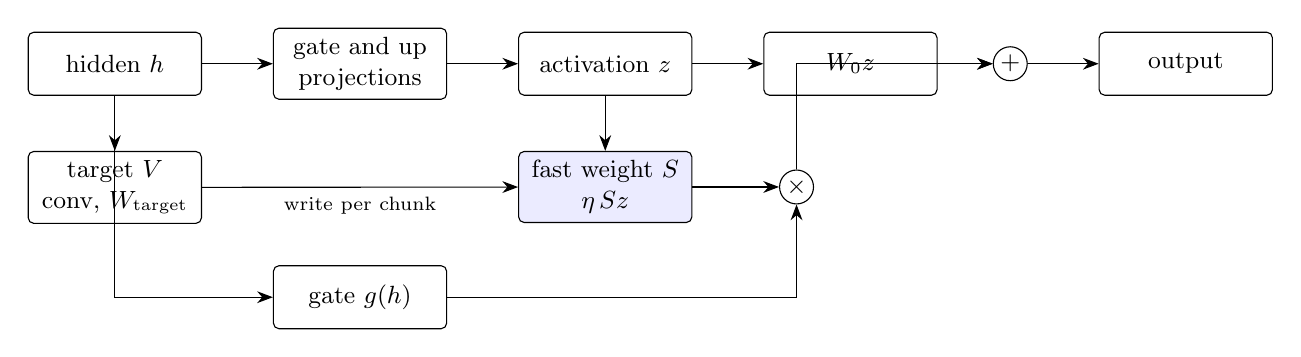
\begin{tikzpicture}[
      node distance=7mm and 9mm,
      box/.style={draw, rounded corners=2pt, minimum height=8mm, minimum width=22mm, align=center, font=\small},
      fast/.style={box, fill=blue!8},
      op/.style={draw, circle, inner sep=1pt, font=\small},
      >={Stealth[length=2mm]}]
    \node[box] (h) {hidden $h$};
    \node[box, right=of h] (gu) {gate and up\\projections};
    \node[box, right=of gu] (z) {activation $z$};
    \node[box, right=of z] (w0) {$W_0 z$};
    \node[fast, below=of z] (s) {fast weight $S$\\$\eta\, S z$};
    \node[box, below=of h] (v) {target $V$\\conv, $W_{\mathrm{target}}$};
    \node[box, below=of gu, yshift=-14mm] (g) {gate $g(h)$};
    \node[op, right=of s, xshift=2mm] (mul) {$\times$};
    \node[op, right=of w0, xshift=-2mm] (add) {$+$};
    \node[box, right=of add] (out) {output};
    \draw[->] (h) -- (gu);
    \draw[->] (gu) -- (z);
    \draw[->] (z) -- (w0);
    \draw[->] (z) -- (s);
    \draw[->] (h) -- (v);
    \draw[->] (v) -- node[below, font=\scriptsize] {write per chunk} (s);
    \draw[->] (h) |- (g);
    \draw[->] (s) -- (mul);
    \draw[->] (g) -| (mul);
    \draw[->] (mul) |- (add);
    \draw[->] (w0) -- (add);
    \draw[->] (add) -- (out);
  \end{tikzpicture}
  \caption{An In-Place TTT layer. The fast weight $S$ is written from the target $V$ and the activation $z$ one chunk at a time, and its contribution is scaled by a learned gate before it is added to the frozen-architecture path $W_0 z$.}
  \label{fig-arch}
\end{figure}

\section{Update rules}

\paragraph{Hebbian.} The Hebbian rule writes an outer product with no error term,
\begin{equation}
  \Delta S_k = \tfrac{1}{C} V_k^\top Z_k, \qquad S_k = S_{\mathrm{carried}} + \textstyle\sum_{j<k} \Delta S_j .
\end{equation}
Nothing in this write checks whether $S$ already predicts $V$, so the state grows with every chunk.

\paragraph{Chunked delta.} The chunked delta rule writes the residual of the current prediction, with the state frozen at the start of each chunk,
\begin{equation}
  \hat V_k = \frac{\eta}{1 + \lVert z \rVert^2}\, Z_k S_k^\top, \qquad \Delta S_k = \tfrac{1}{C} (V_k - \hat V_k)^\top Z_k ,
\end{equation}
with the normalised step $\eta / (1 + \lVert z \rVert^2)$ applied per token row. For this rule the read in Equation~\ref{eq-out} uses the same normalised step, so the TTT term is $\hat V_k$. This is the mini-batch form of the delta rule used by \citet{sun2025learning}, and its error term lets a state that already predicts the target stop growing.

\section{Session persistence}

A session is a sequence of work items, either whole documents or slices of one document. At the end of each item the layer folds the item's total update into a carried state with an exponential moving average,
\begin{equation}
  S_{\mathrm{carried}} \leftarrow \lambda\, S_{\mathrm{carried}} + \Delta S_{\mathrm{item}}, \qquad \lambda = 0.9 ,
\end{equation}
and the next item starts from $S_{\mathrm{carried}}$ instead of from zero. The carried state is detached between items, which limits backpropagation through time to one item. During training every session is a single document, so the carry is learned only between the slices of one document. Carrying it across documents is applied at evaluation, as a test of whether a state learned within documents transfers to the next one. Figure~\ref{fig-persist} contrasts this with resetting.

\begin{figure}[H]
  \centering
  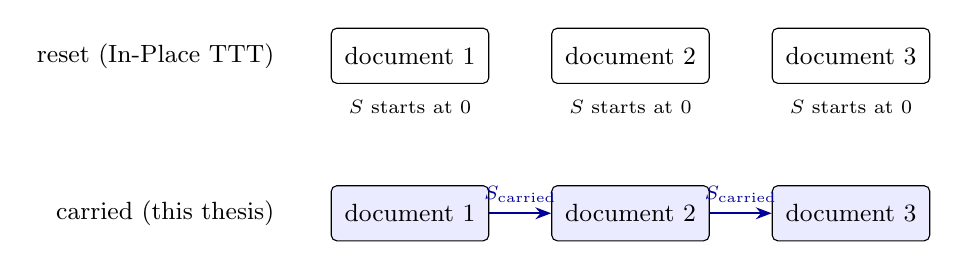
\begin{tikzpicture}[
      doc/.style={draw, rounded corners=2pt, minimum height=7mm, minimum width=20mm, font=\small},
      >={Stealth[length=2mm]}]
    \node[font=\small, anchor=east] at (-0.4,0) {reset (In-Place TTT)};
    \foreach \i in {1,2,3} {
      \node[doc] (a\i) at ({2.8*(\i-1)+1.2},0) {document \i};
      \node[font=\scriptsize] at ({2.8*(\i-1)+1.2},-0.65) {$S$ starts at $0$};
    }
    \node[font=\small, anchor=east] at (-0.4,-2) {carried (this thesis)};
    \foreach \i in {1,2,3} {
      \node[doc, fill=blue!8] (b\i) at ({2.8*(\i-1)+1.2},-2) {document \i};
    }
    \draw[->, thick, blue!60!black] (b1) -- node[above, font=\scriptsize] {$S_{\mathrm{carried}}$} (b2);
    \draw[->, thick, blue!60!black] (b2) -- node[above, font=\scriptsize] {$S_{\mathrm{carried}}$} (b3);
  \end{tikzpicture}
  \caption{Resetting the fast weight at each document, as In-Place TTT does, against carrying it forward with an exponential moving average.}
  \label{fig-persist}
\end{figure}

\section{Stabilisation}

Two mechanisms keep the fast weights stable. A Frobenius norm clip rescales the state whenever it is read, so that $\lVert \eta S \rVert_F \le \tau$ with $\tau = 20$, while preserving its direction. For the Hebbian rule the clip acts only on the read, while for the delta rule the clipped state is also what the next chunk accumulates onto. The output gate is initialised with bias $b_g = -2$, so the TTT term enters at about 12 percent strength at the start of training and the model can learn to open or close it. Separately, the gradients of all trainable parameters are clipped to a total norm of 10. The read-time clip bounds the forward pass, including at evaluation where no gradients exist, while the gradient clip bounds each optimiser step. Chapter~\ref{ch-why} returns to the role of the read-time clip.

\section{Training objective and parameters}

All models are trained with the standard next-token cross-entropy. LoRA adapters are trained in every model, so that the TTT models and the control differ only in the TTT layers. The TTT models additionally train the down-projection $W_0$ of the TTT layers and the new modules (target projection, convolution and gate). Counted from the layer shapes of Qwen3-0.6B, this gives about 68.0 million trainable parameters for a TTT model (9.2 million LoRA, 44.0 million in the 14 down-projections, 14.8 million in the new modules) against about 10.1 million for the LoRA-only control. This difference matters for interpreting the results and is discussed in Chapters~\ref{ch-q1} and~\ref{ch-limits}.

\section{Implementation}

The system is implemented in Python with PyTorch, Hugging Face Transformers and PEFT, and runs on cloud GPUs through Modal. It is organised in rings with inward-only dependencies, so that the training loop, the carry lifecycle and the evaluation suites run against in-memory fakes and are covered by a fast test suite without a GPU. Every evaluation writes a self-describing bundle of raw per-document rows, tables, figures and a manifest recording the exact configuration and code version, and every table and figure in this thesis is regenerated from those bundles without a GPU.

% ======================================================================
\chapter{Experimental Setup and Evaluation Protocol}
\label{ch-eval}

\section{Model and data}

All models start from the pretrained Qwen3-0.6B model. TTT layers replace the MLPs of the 14 odd-numbered layers, 1, 3 and so on up to 27. Training and evaluation use the SlimPajama-6B subset \citep{yoon2023slimpajama6b} of SlimPajama \citep{soboleva2023slimpajama}, restricted to six RedPajama sources, namely ArXiv, Book, C4, Github, StackExchange and Wikipedia. Training uses 4000 documents of at least 2048 tokens, truncated to 16384 tokens and balanced across sources towards a target mix of 25 percent C4, 20 percent each of Github and ArXiv, 15 percent Book, and 10 percent each of Wikipedia and StackExchange. Each session is one document, read whole if shorter than 2100 tokens and otherwise split into two to six slices of at least 1000 tokens.

\section{Training}

All runs use LoRA of rank 16 with $\alpha = 32$ and dropout 0.05, a LoRA learning rate of $10^{-5}$, AdamW, 16 gradient accumulation steps, a warmup of 2 percent of steps, cosine decay over the full epoch of 1050 optimiser steps, and seed 42. TTT runs train their down-projections at $3 \times 10^{-5}$ and their new modules at $6 \times 10^{-2}$. Checkpoints at steps 200, 400 and 600 are evaluated. Because the epoch length depends only on the data and the session strategy, all runs share the same 1050-step schedule and data order. Appendix~\ref{app-hparams} lists every setting.

\section{Models compared}

\begin{description}
  \item[LoRA-only.] The matched control, with no TTT layers.
  \item[Hebbian.] TTT layers with the Hebbian rule.
  \item[Delta.] TTT layers with the chunked delta rule.
\end{description}

\section{Held-out data}

The held-out set is drawn from documents never used in training. It is drawn from the last 15{,}000 rows of the dataset, which are removed before any training stage, and long enough to cut into slices. It has 20 documents per source, except Book, which is rare in the subset and yields only 6, giving 106 documents and 656{,}331 tokens. Every model is evaluated on exactly the same documents.

\section{Evaluation regimes}

Each document is cut into 8 equal slices and measured in four regimes (Table~\ref{tab-regimes}).

\begin{table}[H]
  \centering
  \caption{Evaluation regimes, each measured on every held-out document.}
  \label{tab-regimes}
  \begin{tabular}{llll}
    \toprule
    Regime & LoRA & Fast-weight updates & Carried between slices \\
    \midrule
    base & off & off, pretrained $W_0$ & no \\
    TTT off & on & off & no \\
    TTT, reset per slice & on & on & no \\
    TTT, carried & on & on & yes \\
    \bottomrule
  \end{tabular}
\end{table}

Differences between regimes give the decomposition reported throughout.
\begin{description}
  \item[Training gain.] Base minus TTT off. Everything the slow weights learned, including LoRA and, for TTT models, the trained $W_0$.
  \item[Within-document gain.] TTT off minus TTT reset per slice. What the fast weights learn inside a slice.
  \item[Between-slice gain.] TTT reset per slice minus TTT carried. What carrying state from earlier slices of the same document adds.
  \item[Matched gain.] The LoRA-only model minus the TTT model with its fast weights carried. The total advantage over the control.
\end{description}

\section{Persistence suites}

Three further suites probe persistence directly.
\begin{description}
  \item[Boundary.] For each source, a chain of five documents is read under three arms, carrying state across documents, resetting at document boundaries, and resetting at every slice. The cross-document gain compares the first two arms on documents two to five of each chain (24 documents), and the cross-slice gain compares the last two on all 30 documents. The arm that resets at document boundaries is exactly the setting of In-Place TTT, so the cross-document gain is a direct comparison of our persistent method against a reimplementation of In-Place TTT on the same model, data and documents.
  \item[Repeat.] Each document is read ten times in a row with its carried state never reset. Each later reading is compared with the first, and the tenth reading is also compared with the second, which tests whether the carry keeps compounding after one exposure. This is the most favourable test possible for a carried state, since the state was built from the very document being read again.
  \item[Swap.] A target document is read after the state has been primed on two documents from the same source or from a different source, each read whole, and compared with reading it unprimed, to test whether any carried benefit is source-specific, as planned in the proposal.
\end{description}

\section{Statistics}

Perplexity within a document is token-weighted over its slices. A gap between two regimes is the difference of their geometric-mean perplexities over documents, positive when the second regime has lower perplexity. We report 95 percent percentile bootstrap intervals from 1000 resamples of documents, with both regimes resampled on the same indices, and the win rate, the fraction of documents on which the second regime is lower. A star marks an interval that excludes zero. Following \citet{meister2021beyond}, every result is reported as an effect size with its interval rather than as a significance test alone.

\section{Measurement integrity}

Two errors in the evaluation pipeline were found and fixed during the study, and both are reported for transparency. First, the in-training evaluation ran with LoRA dropout active, which perturbed every regime slightly. The final evaluation runs in evaluation mode, and no reported number used the in-training evaluation. Second, the base regime initially kept the trained $W_0$ of the TTT layers instead of the pretrained one, which understated the training gain of TTT models. The fixed pipeline restores the pretrained $W_0$, and earlier bundles were corrected by taking the base regime from the LoRA-only bundle, which contains the true base model on the same documents. Two sanity checks confirm the pipeline. The LoRA-only model, which has no fast weights, gives a within-document and between-slice gain of exactly 0.000 at every step, and the base-model perplexities are identical across all LoRA-only bundles.

% ======================================================================
\chapter{Results for Q1, the Contribution of Carry}
\label{ch-q1}

\section{Overall performance}

Figure~\ref{fig-absolute} shows the held-out perplexity of each model. All three improve substantially on the base model, whose geometric-mean perplexity is 12.838, and at every checkpoint the delta model is best, the Hebbian model second and the LoRA-only control third.

\begin{figure}[H]
  \centering
  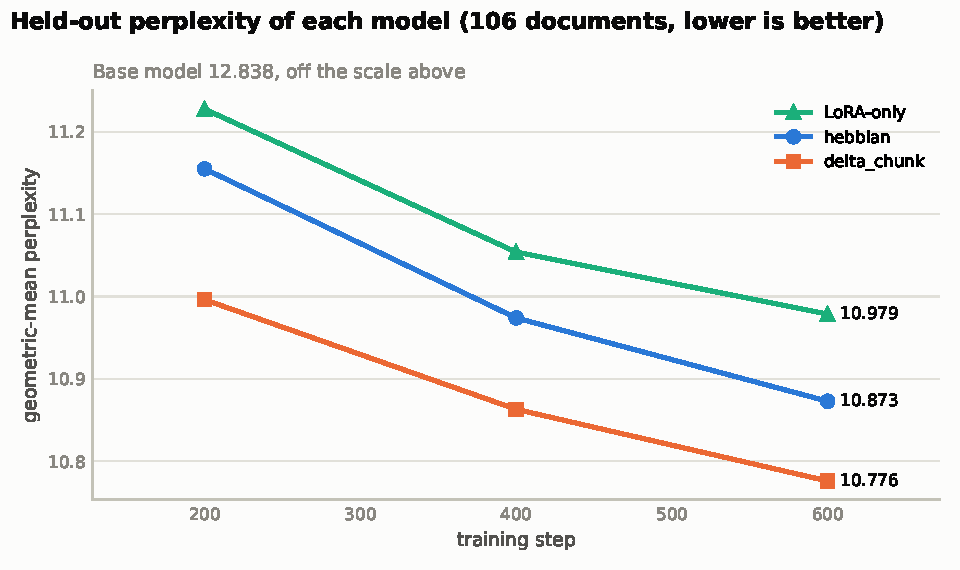
\includegraphics[width=0.8\linewidth]{figures/F5_absolute_ppl.pdf}
  \caption{Geometric-mean held-out perplexity of each model by training step. The base model is at 12.838.}
  \label{fig-absolute}
\end{figure}

\begin{table}[H]
  \centering
  \caption{Gains in perplexity on 106 held-out documents. Positive values mean lower perplexity. A star marks a 95 percent interval that excludes zero. Full intervals are in Appendix~\ref{app-full}.}
  \label{tab-main}
  \small
  \begin{tabular}{llrrrr}
    \toprule
    Step & Model & Training gain & Within-document & Cross-document & Matched gain \\
    \midrule
    \multirow{3}{*}{200} & LoRA-only & $+1.610$\sig & $0$ & n/a & n/a \\
     & Hebbian & $+1.653$\sig & $+0.016$\sig & $+0.008$ & $+0.073$\sig \\
     & Delta & $+1.670$\sig & $+0.144$\sig & $+0.003$ & $+0.232$\sig \\
    \midrule
    \multirow{3}{*}{400} & LoRA-only & $+1.784$\sig & $0$ & n/a & n/a \\
     & Hebbian & $+1.852$\sig & $+0.014$\sig & $-0.003$ & $+0.080$\sig \\
     & Delta & $+1.909$\sig & $+0.059$\sig & $+0.006$ & $+0.191$\sig \\
    \midrule
    \multirow{3}{*}{600} & LoRA-only & $+1.859$\sig & $0$ & n/a & n/a \\
     & Hebbian & $+1.928$\sig & $+0.034$\sig & $-0.004$ & $+0.106$\sig \\
     & Delta & $+1.992$\sig & $+0.058$\sig & $-0.002$ & $+0.203$\sig \\
    \bottomrule
  \end{tabular}
\end{table}

\begin{figure}[H]
  \centering
  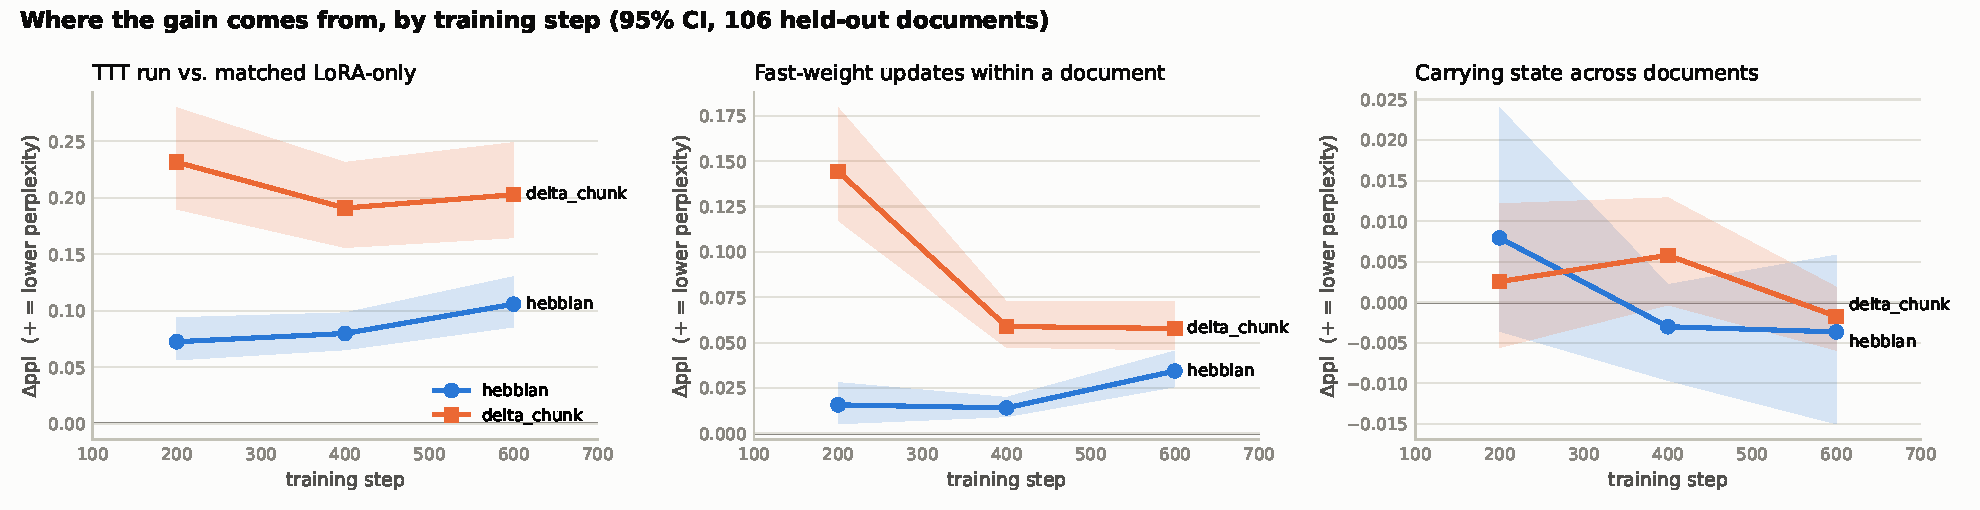
\includegraphics[width=\linewidth]{figures/F1_gains_vs_step.pdf}
  \caption{Gains by training step with 95 percent bootstrap bands. Left, the TTT model against the matched LoRA-only control. Middle, fast-weight updates within a document. Right, state carried across document boundaries. Each panel has its own scale.}
  \label{fig-gains}
\end{figure}

\section{TTT models beat the matched control, mostly through capacity}

Both TTT models are better than the LoRA-only control at every checkpoint (Table~\ref{tab-main}, Figure~\ref{fig-gains}). The Hebbian model leads by 0.073 to 0.106 perplexity and the delta model by 0.191 to 0.232, and at step 600 both are better on all 106 documents.

Most of this lead is not test-time learning. A TTT model trains about 6.7 times as many parameters as the control, and its training gain, measured with the fast weights switched off, already exceeds that of the control (1.928 and 1.992 against 1.859 at step 600). At step 600 the Hebbian model's lead of 0.106 splits into 0.069 of extra training gain, 0.034 of within-document gain and 0.002 between slices, so about two thirds is capacity. The delta model's lead of 0.203 splits into 0.133, 0.058 and 0.012, the same proportion.

\section{Fast weights help within a document}

Switching the fast weights on inside a slice lowers perplexity at every checkpoint for both rules, on 72 to 100 percent of documents. The delta rule's within-document gain is 9 times the Hebbian gain at step 200, 4 times at step 400 and 1.7 times at step 600. It is largest early, 0.144 at step 200 and 0.276 at step 100, and settles near 0.06, which is consistent with the slow weights absorbing part of what the fast weights first provided.

The gain does not build up along a document (Figure~\ref{fig-position}). It is already present in the first slice, dips in the middle slices and shows no upward trend, so the fast weights adapt locally rather than accumulating knowledge of the document. Carrying state from earlier slices of the same document adds a small gain for the delta rule, 0.012 at step 600 and about 0.015 per slice from the second slice on. This is the only form of persistence found to help.

\begin{figure}[H]
  \centering
  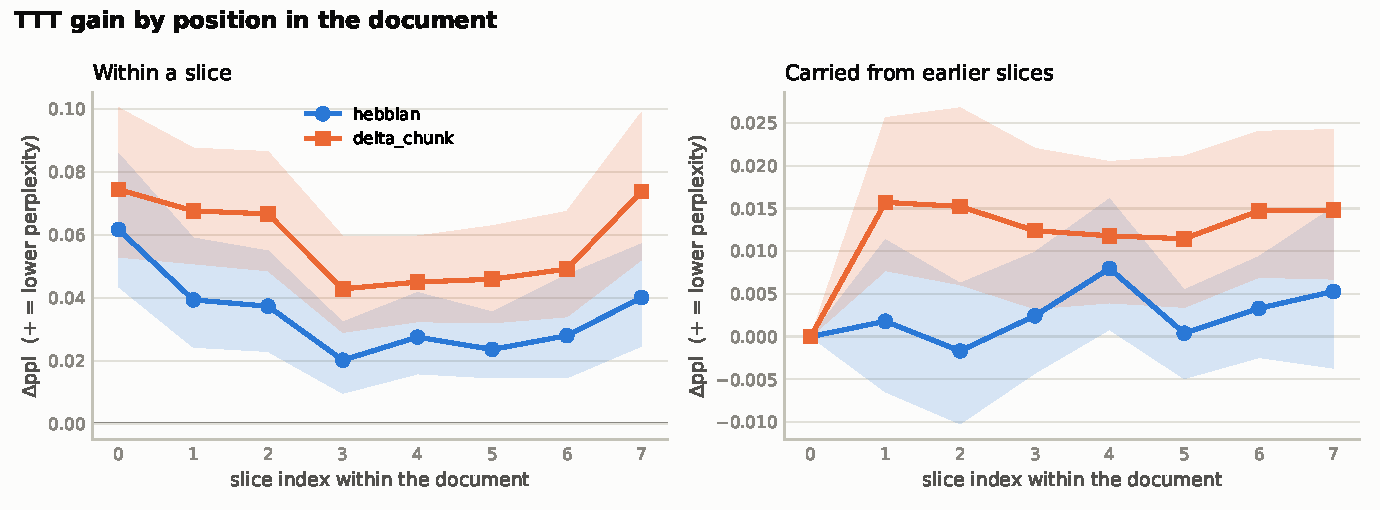
\includegraphics[width=\linewidth]{figures/F2_by_position.pdf}
  \caption{Gains at step 600 by slice index, with 95 percent bootstrap bands. Left, fast-weight updates within a slice. Right, state carried from earlier slices, zero at the first slice by construction.}
  \label{fig-position}
\end{figure}

\section{Carrying state across documents contributes nothing}

The cross-document gain lies between $-0.004$ and $+0.008$ perplexity at every checkpoint for both rules, and every interval includes zero (Table~\ref{tab-main}, Figure~\ref{fig-gains} right). Three times more training does not move it. Since the reset arm of the boundary suite is the In-Place TTT setting, this is also the comparison with In-Place TTT. On the same model, data and documents, session persistence adds nothing to a reimplementation of In-Place TTT.

Table~\ref{tab-persist} collects the persistence measures at step 600. Re-reading a document with its own carried state never helps. Against the first reading, the gain of every later reading up to the tenth is within 0.002 perplexity, and no interval excludes zero, for either rule (Figure~\ref{fig-repeat}). The tenth reading against the second is $+0.000$ with an interval of $\pm 0.001$ for both rules, even though the carried state was built from that very document. The swap suite (Figure~\ref{fig-swap}) shows that a foreign carried state can do harm. For the Hebbian model, a state primed on a different source raises perplexity in 15 of the 30 source pairs, by 0.022 on average and by up to 0.07, and never lowers it significantly, while same-source priming is close to neutral ($-0.008$). The Hebbian same-against-other effect of 0.010 in Table~\ref{tab-persist} therefore reflects a foreign state hurting less, not a same-source state helping. For the delta model, priming is neutral in either case, with 3 of 30 pairs significant in mixed directions. No carried state helps the next document.

\begin{table}[H]
  \centering
  \caption{Persistence measures at step 600, pooled over sources, with 95 percent bootstrap intervals.}
  \label{tab-persist}
  \small
  \begin{tabular}{lrrr}
    \toprule
    Measure & Documents & Hebbian & Delta \\
    \midrule
    Cross-document & 24 & $-0.004$ {\footnotesize [$-0.015$, $+0.006$]} & $-0.002$ {\footnotesize [$-0.006$, $+0.002$]} \\
    Cross-slice & 30 & $+0.005$ {\footnotesize [$-0.001$, $+0.014$]} & $+0.015$\sig {\footnotesize [$+0.005$, $+0.029$]} \\
    Tenth reading against second & 106 & $+0.000$ {\footnotesize [$-0.001$, $+0.001$]} & $+0.000$ {\footnotesize [$-0.001$, $+0.001$]} \\
    Same against other source & 30 & $+0.010$\sig {\footnotesize [$+0.004$, $+0.018$]} & $+0.002$ {\footnotesize [$-0.000$, $+0.004$]} \\
    \bottomrule
  \end{tabular}
\end{table}

\begin{figure}[H]
  \centering
  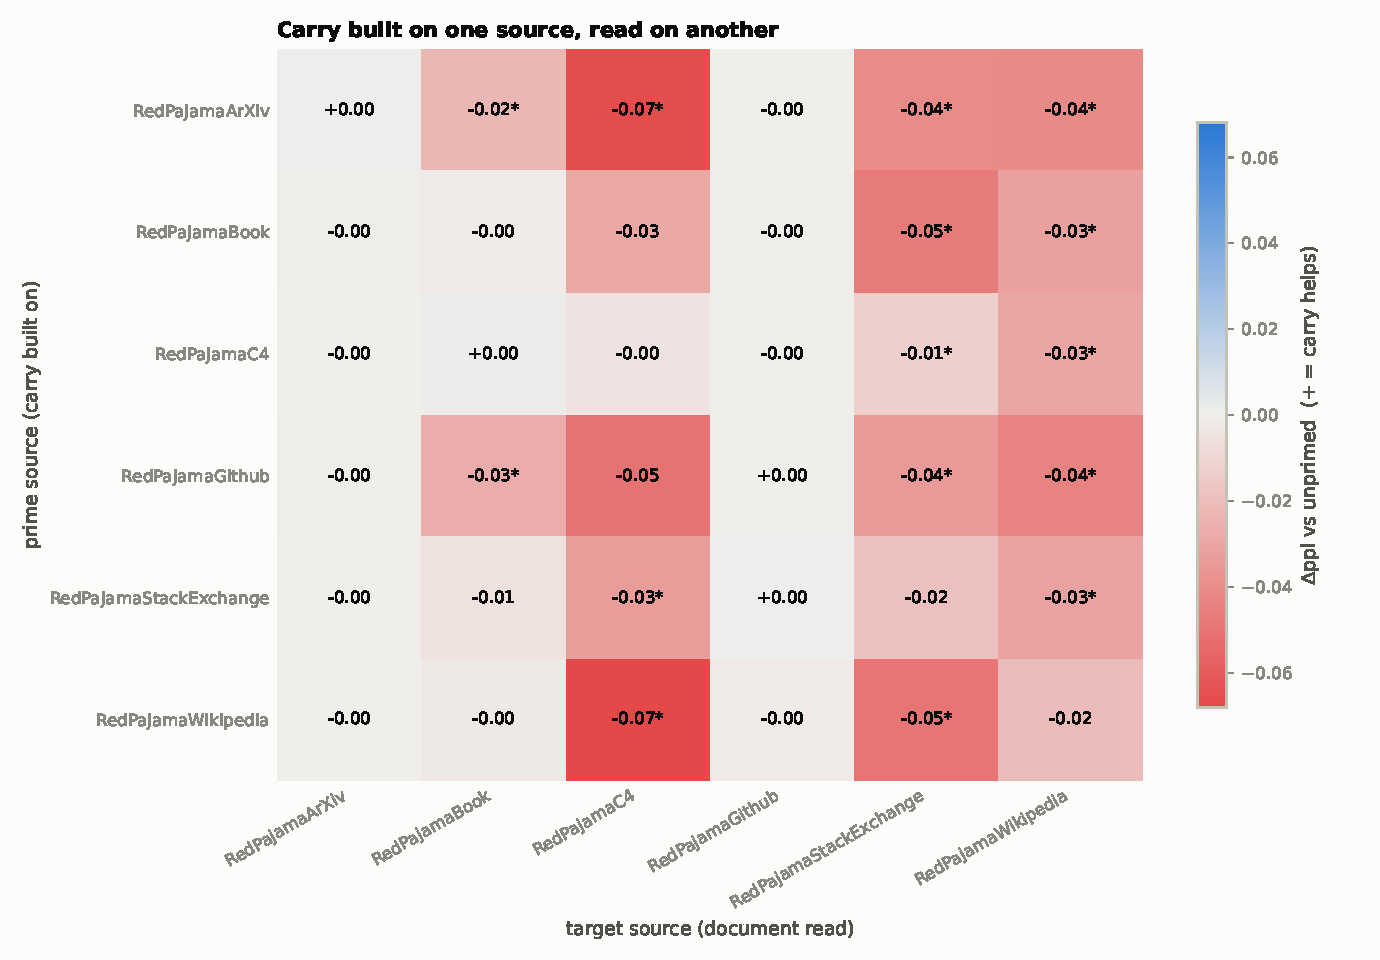
\includegraphics[width=0.49\linewidth]{figures/F9_swap_hebbian.pdf}\hfill
  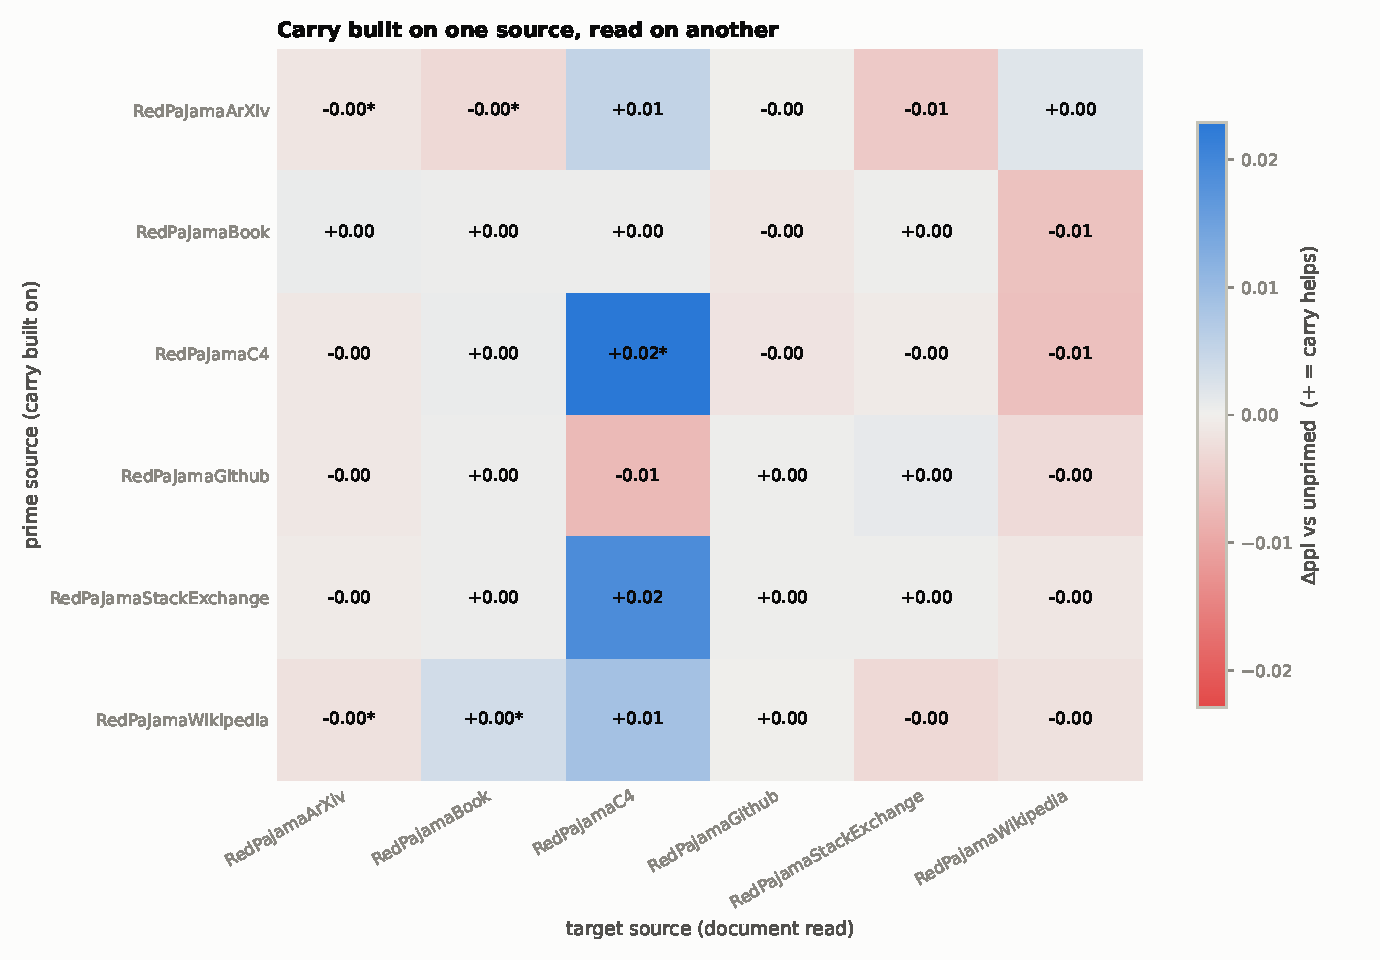
\includegraphics[width=0.49\linewidth]{figures/F9_swap_delta_chunk.pdf}
  \caption{State primed on one source (rows) and read on another (columns), against an unprimed read, at step 600, five target documents per cell. Left, Hebbian. Right, delta. Negative values mean the primed state made perplexity worse.}
  \label{fig-swap}
\end{figure}

\section{Answer to Q1}

Carry, in the sense of information retained from the previous document, contributes nothing measurable to language model improvement in this setting, where the carry is learned within documents and applied across them. The improvement of a TTT model over a matched baseline comes from extra trainable capacity and from adaptation within each document, and the only persistence that helps is carrying state between slices of the same document with the delta rule. Chapter~\ref{ch-design} revisits this answer with a redesigned carry, which makes the carry between slices of the same document substantially useful, and which after full training is harmful across unrelated documents.

% ======================================================================
\chapter{Results for Q2, Domains}
\label{ch-q2}

\section{Per-source gains}

Table~\ref{tab-sources} gives the gains per source at step 600. In absolute perplexity, the lead over the control is largest on C4, Wikipedia and Book, the sources the base model finds hardest. In relative terms, which divide by each source's perplexity and so compare sources fairly, StackExchange benefits most for both rules, and ArXiv, Book and Github least.

\begin{table}[H]
  \centering
  \caption{Per-source gains at step 600. Absolute gains in perplexity, relative gains in percent of the reference perplexity. All intervals exclude zero except the Hebbian within-document gain on Book.}
  \label{tab-sources}
  \small
  \begin{tabular}{lrrrrrr}
    \toprule
    & & \multicolumn{2}{c}{Within-document} & \multicolumn{2}{c}{Matched gain} & \\
    \cmidrule(lr){3-4} \cmidrule(lr){5-6}
    Source & Base ppl & Hebbian & Delta & Hebbian & Delta & Documents \\
    \midrule
    ArXiv & 7.45 & $+0.004$ (0.07\%) & $+0.029$ (0.45\%) & $+0.053$ (0.81\%) & $+0.098$ (1.52\%) & 20 \\
    Book & 29.30 & $+0.022$ (0.09\%) & $+0.083$ (0.35\%) & $+0.172$ (0.72\%) & $+0.331$ (1.39\%) & 6 \\
    C4 & 37.40 & $+0.064$ (0.21\%) & $+0.161$ (0.53\%) & $+0.247$ (0.81\%) & $+0.536$ (1.76\%) & 20 \\
    Github & 4.79 & $+0.005$ (0.11\%) & $+0.016$ (0.37\%) & $+0.028$ (0.65\%) & $+0.066$ (1.53\%) & 20 \\
    StackExchange & 9.47 & $+0.067$ (0.83\%) & $+0.059$ (0.74\%) & $+0.131$ (1.62\%) & $+0.217$ (2.68\%) & 20 \\
    Wikipedia & 21.53 & $+0.075$ (0.42\%) & $+0.111$ (0.62\%) & $+0.183$ (1.00\%) & $+0.345$ (1.89\%) & 20 \\
    \bottomrule
  \end{tabular}
\end{table}

Figure~\ref{fig-heat} shows how these relative gains develop over training. The delta rule helps every source at every step, while the Hebbian rule's within-document gain only becomes reliable on most sources by step 600. The ordering of sources is fairly stable across steps.

\begin{figure}[H]
  \centering
  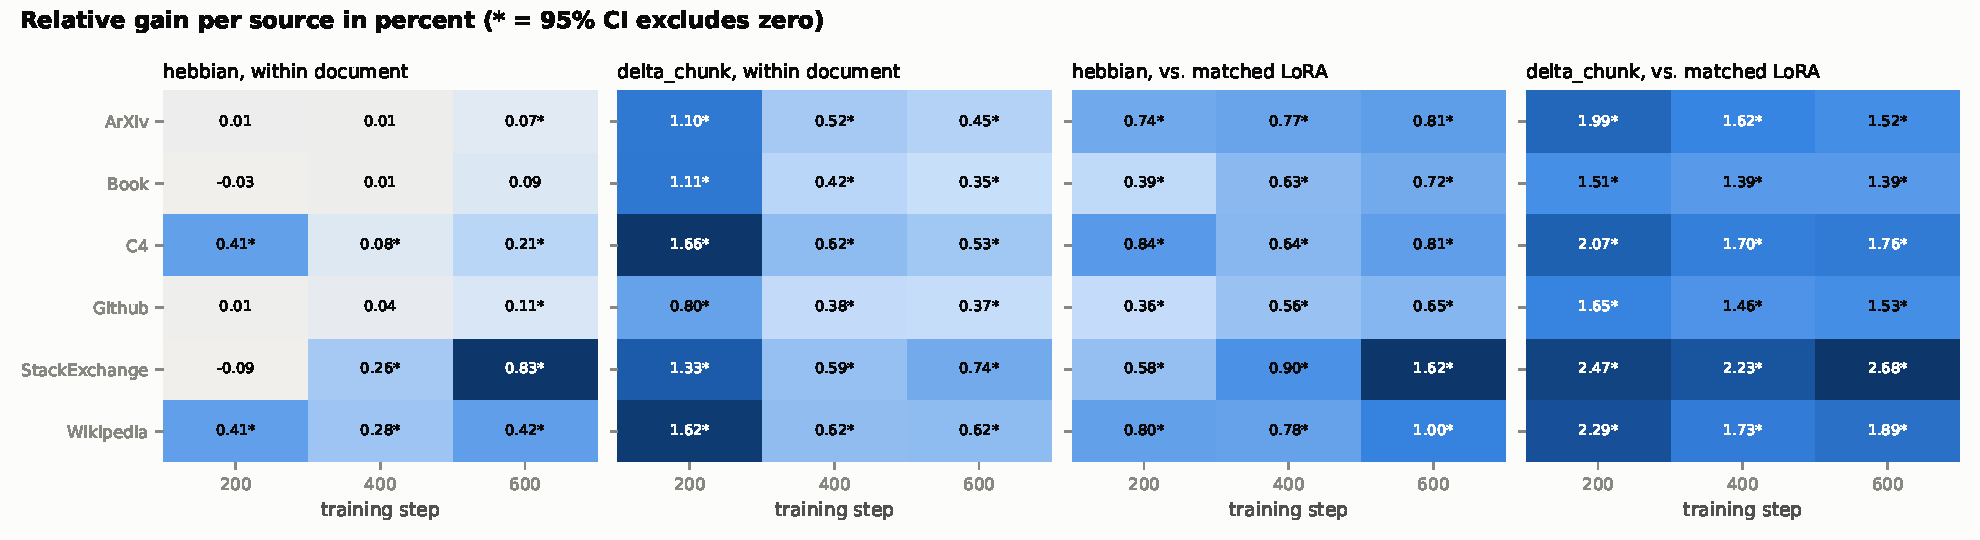
\includegraphics[width=\linewidth]{figures/F6_source_heatmaps.pdf}
  \caption{Relative gain per source and step, in percent of the reference perplexity, for the within-document gain and the lead over the matched control. Each panel has its own colour scale, so compare cells within a panel and read the printed values across panels.}
  \label{fig-heat}
\end{figure}

\section{Is domain difficulty the explanation}

A natural hypothesis is that test-time adaptation helps most where the base model struggles most. Figure~\ref{fig-domain} tests this by plotting each source's relative within-document gain against its base perplexity. The rank correlation is weak, $\rho = +0.20$ for the Hebbian rule and $+0.09$ for the delta rule over six sources, so difficulty does not predict the gain. StackExchange, a source of moderate difficulty, benefits most. A plausible reading, not tested here, is that question-and-answer threads repeat local terminology within a document, which is exactly what a chunk-level fast weight can exploit. With six sources the correlation is descriptive only.

\begin{figure}[H]
  \centering
  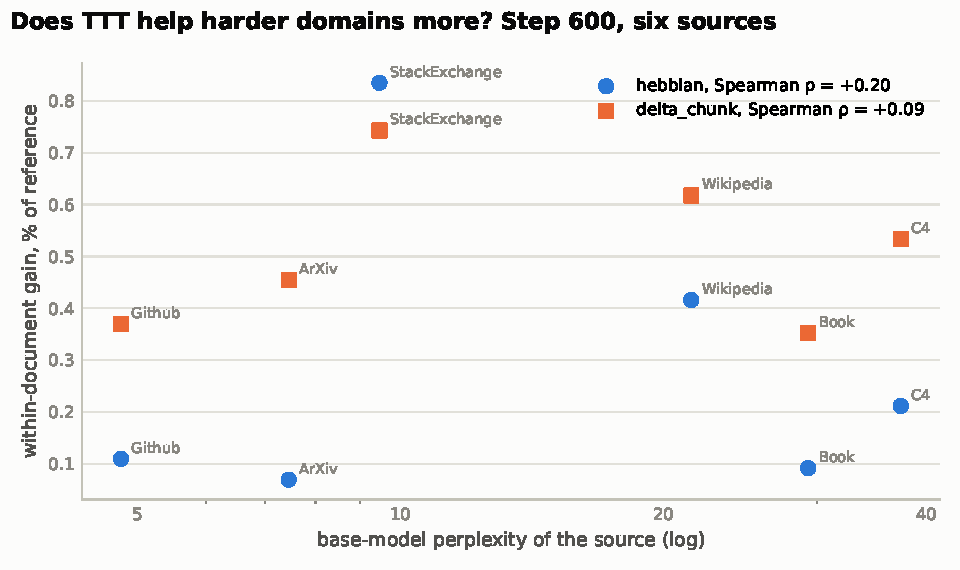
\includegraphics[width=0.8\linewidth]{figures/F7_domain_correlates.pdf}
  \caption{Relative within-document gain at step 600 against the base-model perplexity of each source.}
  \label{fig-domain}
\end{figure}

\section{Carry across domains}

No source shows a reliable benefit from carrying state across documents (Figure~\ref{fig-sources}). Per-source cross-document estimates rest on four documents each, and the only two whose intervals exclude zero, Hebbian on Book and delta on Wikipedia, are both negative and should be read as noise among twelve tests.

\begin{figure}[H]
  \centering
  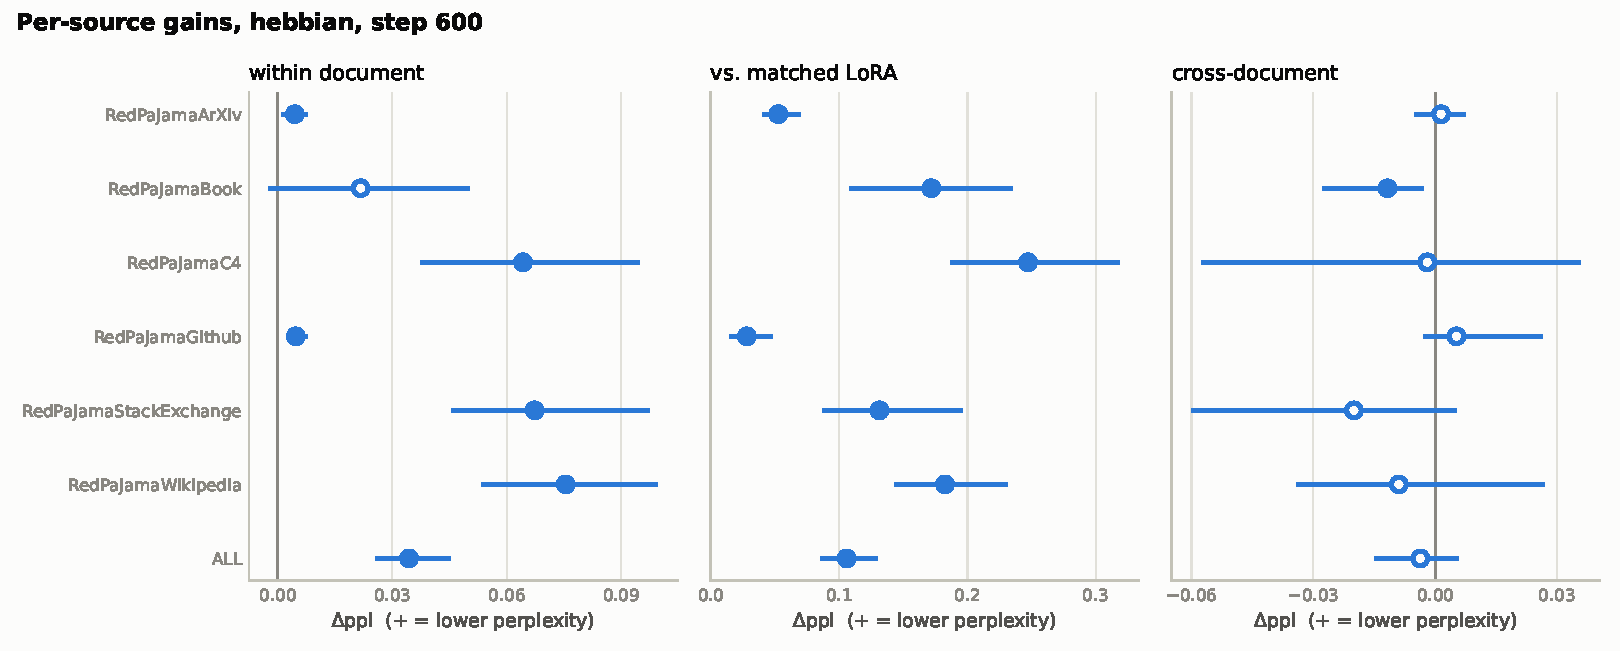
\includegraphics[width=\linewidth]{figures/F4_per_source_hebbian.pdf}\\[4pt]
  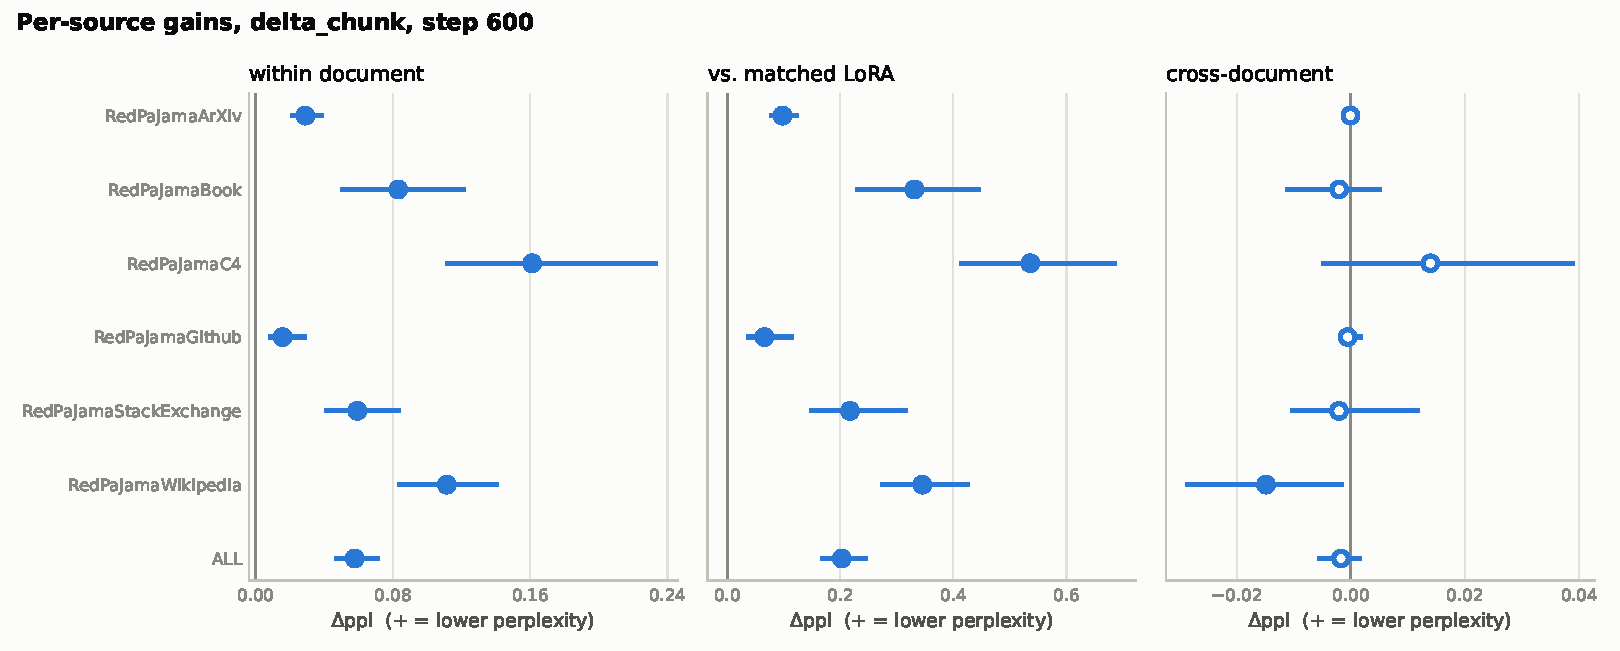
\includegraphics[width=\linewidth]{figures/F4_per_source_delta_chunk.pdf}
  \caption{Per-source gains at step 600 for the Hebbian model (top) and the delta model (bottom). A filled marker means the 95 percent interval excludes zero.}
  \label{fig-sources}
\end{figure}

\section{Answer to Q2}

For within-document adaptation, StackExchange and Wikipedia benefit most in relative terms and ArXiv, Book and Github least, and the delta rule helps every domain. The differences are not explained by how hard a domain is for the base model. For session-persistent carry, the subject of Q2, no domain performs well, because the carry contributes nothing in any domain.

% ======================================================================
\chapter{Why Persistence Fails}
\label{ch-why}

\section{The read-time clip is always active}

The clip binds whenever $\lVert \eta S \rVert_F > \tau$. In units of the pretrained down-projection, this is a state ratio $\lVert \eta S \rVert_F / \lVert W_0 \rVert_F$ above $\tau / \lVert W_0 \rVert_F = 0.43$, given a mean $\lVert W_0 \rVert_F$ of 46.6 over the TTT layers. Across every boundary, repeat, swap and regime measurement at steps 200, 400 and 600, the state ratio is above this threshold on 100 percent of measurements, by a factor of at least 255 for the Hebbian model and at least 1597 for the delta model (Table~\ref{tab-clip}, Figure~\ref{fig-dist}).

\begin{table}[H]
  \centering
  \caption{Fraction of measurements on which the read-time clip is active, and the smallest margin by which the state exceeds the clip threshold of 0.43.}
  \label{tab-clip}
  \small
  \begin{tabular}{llrrr}
    \toprule
    Model & Step & Measurements & Clip active & Smallest margin \\
    \midrule
    Hebbian & 200 & 826 & 100\% & $843\times$ \\
    Hebbian & 400 & 826 & 100\% & $292\times$ \\
    Hebbian & 600 & 2096 & 100\% & $255\times$ \\
    Delta & 200 & 826 & 100\% & $2478\times$ \\
    Delta & 400 & 826 & 100\% & $1900\times$ \\
    Delta & 600 & 2096 & 100\% & $1597\times$ \\
    \bottomrule
  \end{tabular}
\end{table}

\begin{figure}[H]
  \centering
  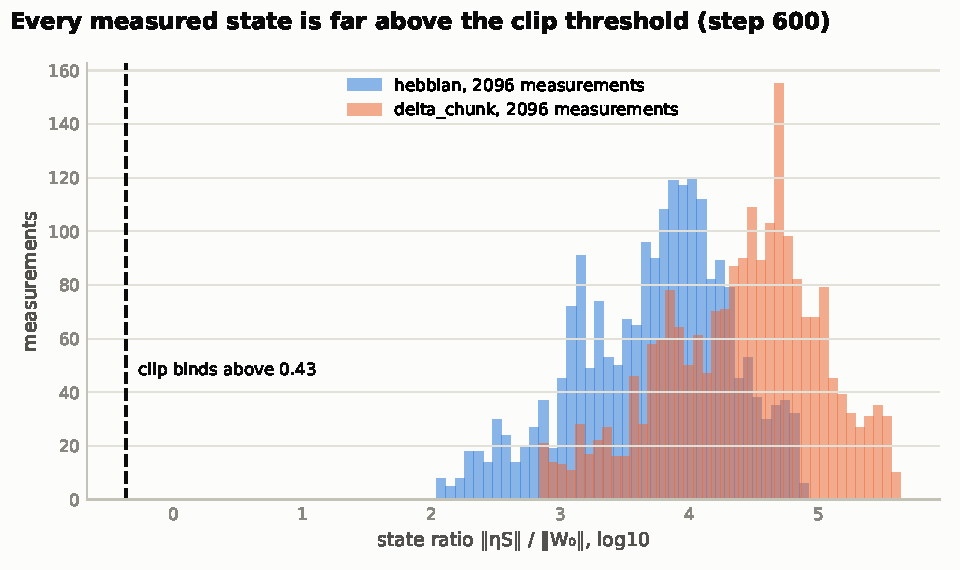
\includegraphics[width=0.8\linewidth]{figures/F10_state_distribution.pdf}
  \caption{Distribution of the state ratio over all measurements at step 600, on a log scale, with the clip threshold dashed.}
  \label{fig-dist}
\end{figure}

\section{Only the direction of the state reaches the output}

A saturated clip means that the magnitude of the state never reaches the output. What reaches it is a vector of norm $\tau$ pointing along the accumulated state. Two observations follow. First, re-reading a document grows the carried state by a factor of about 6.5 over ten readings, from a median state ratio of about 14{,}600 after the first reading to about 95{,}000 after the tenth for the delta model, and from about 2{,}600 to 16{,}900 for the Hebbian model, while perplexity stays flat (Figure~\ref{fig-repeat}, which starts at the second reading). Second, carrying state into a new document makes it about two to four times larger than a state reset at the boundary, again with no effect on perplexity (Figure~\ref{fig-chain}). With $\lambda = 0.9$ the carried direction is an average over earlier documents, and once normalised to $\tau$ it holds nothing specific to the next one.

\begin{figure}[H]
  \centering
  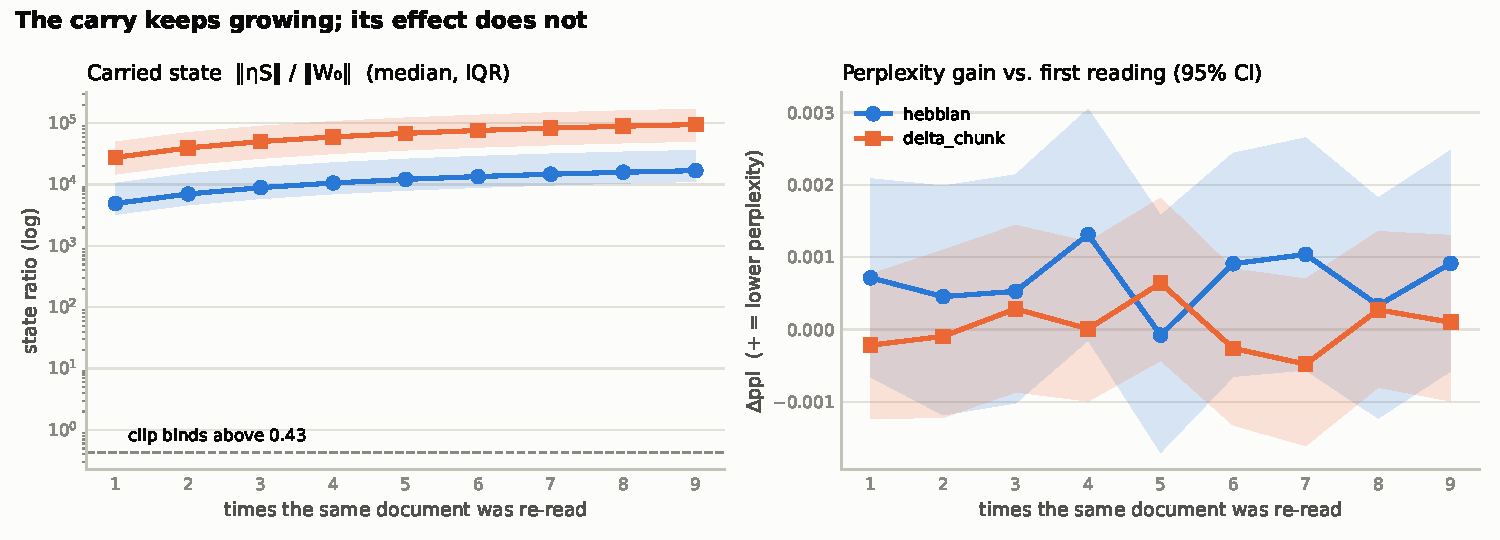
\includegraphics[width=\linewidth]{figures/F3_repeat_mechanism.pdf}
  \caption{Repeated reading of the same document at step 600. Left, the carried state relative to $\lVert W_0 \rVert_F$ on a log scale, with the clip threshold dashed. Right, the perplexity gain against the first reading.}
  \label{fig-repeat}
\end{figure}

\begin{figure}[H]
  \centering
  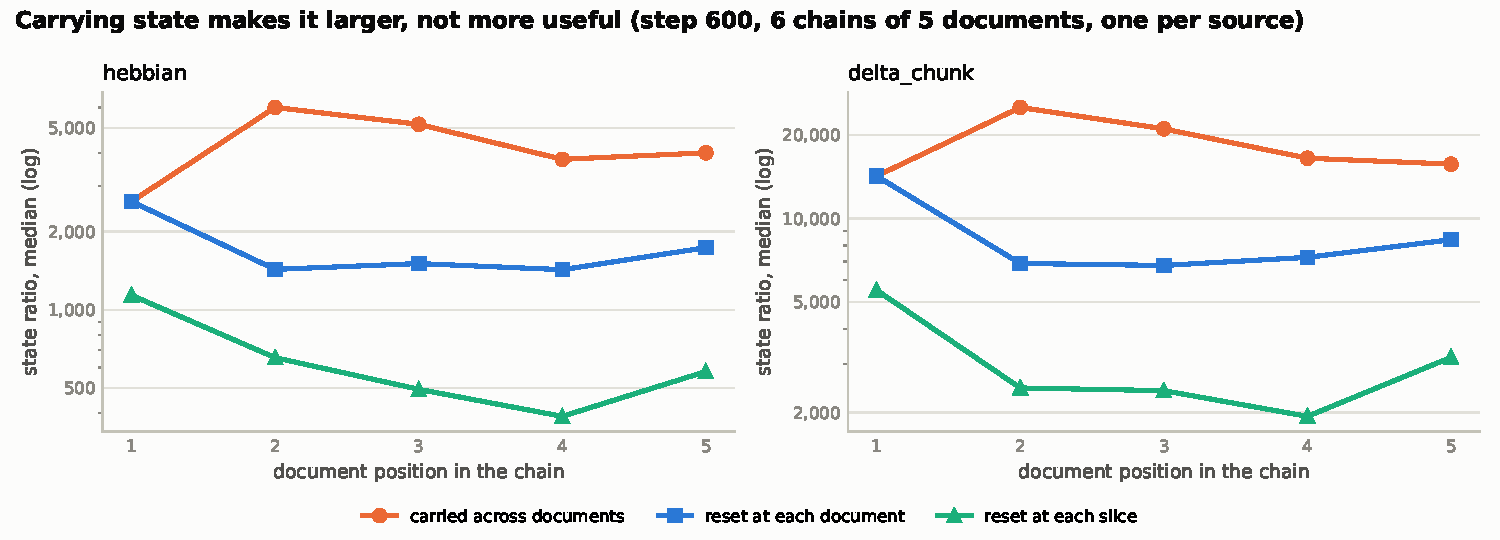
\includegraphics[width=\linewidth]{figures/F8_chain_states.pdf}
  \caption{Median state ratio along chains of five documents at step 600, under the three boundary arms.}
  \label{fig-chain}
\end{figure}

\section{Removing the clip does not help}

If saturation erases the information in the state's magnitude, removing the clip might let persistence work. We trained both rules without the clip, keeping every other setting, the data order and the gradient clip (Figure~\ref{fig-noclip}).

The Hebbian model collapses. It settles at a training loss of about 8.1, a perplexity of roughly 3300, and does not recover within the 200 steps run, while the clipped Hebbian model trains normally. Its early loss, 25.8 over the first 10 steps, is not by itself evidence, because a clipped Hebbian model can also start with a loss spike that it recovers from (Chapter~\ref{ch-design}). The unclipped delta model, reading the same data in the same order, stays between 1.8 and 2.8 throughout. Without an error term and with a fixed step, the Hebbian state grows with every chunk and wrecks the forward pass.

\begin{figure}[H]
  \centering
  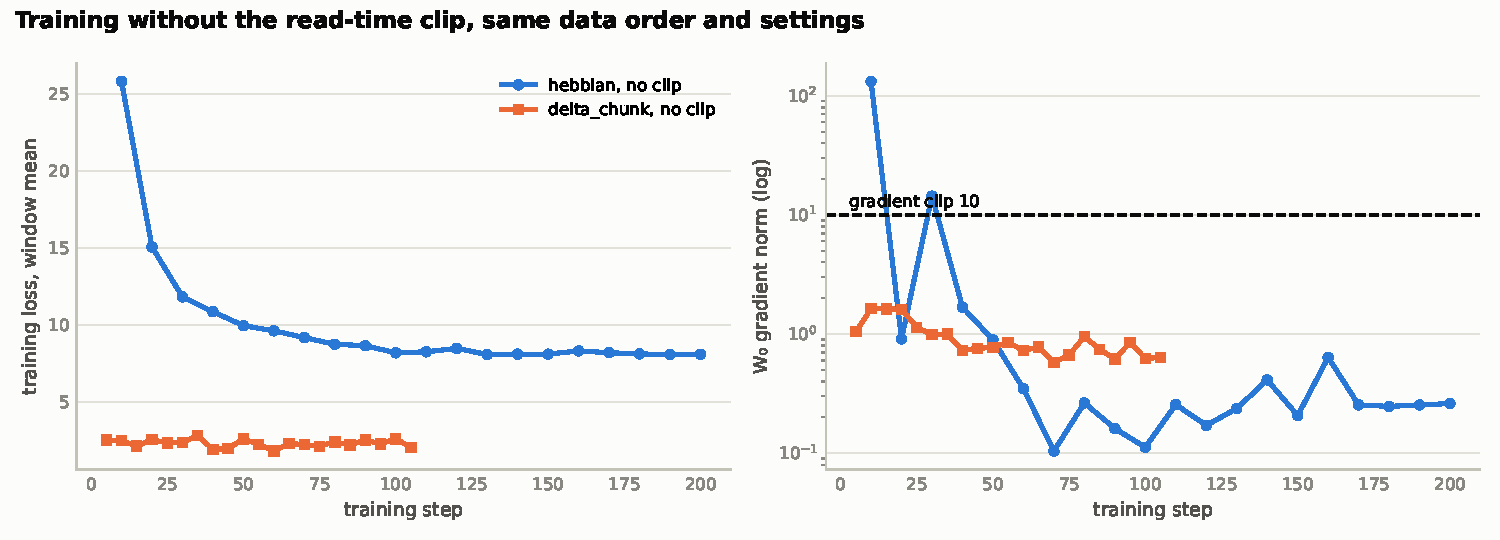
\includegraphics[width=\linewidth]{figures/F11_noclip_training.pdf}
  \caption{Training without the read-time clip, Hebbian to step 200 and delta to step 105, with the same data order. Left, training loss averaged over each logging window. Right, gradient norm of the TTT down-projections at each logged step, on a log scale, with the gradient clip dashed.}
  \label{fig-noclip}
\end{figure}

The delta model trains with a normal loss, but it does so by switching the fast weights off (Table~\ref{tab-noclip}). By step 100 its output gate has closed completely, with a median of 0.00 against 0.92 for the clipped model at the same step. Every TTT effect is zero, and the model as a whole is worse than its clipped counterpart by 0.167 perplexity on all 106 documents. Even without the clip its state is about 2000 times the clip threshold, far beyond any scale the model can use.

\begin{table}[H]
  \centering
  \caption{The delta model at step 100 with and without the read-time clip, on the same 106 documents.}
  \label{tab-noclip}
  \small
  \begin{tabular}{lrr}
    \toprule
    Measure & With clip & Without clip \\
    \midrule
    Within-document gain & $+0.276$\sig & $+0.003$ \\
    Between-slice gain & $+0.051$\sig & $+0.002$ \\
    Cross-document gain & $-0.002$ & $-0.005$ \\
    Cross-slice gain & $+0.062$\sig & $+0.004$ \\
    Output gate, median & $0.92$ & $0.00$ \\
    State ratio, median & $\approx 73{,}600$ & $\approx 890$ \\
    Full model, without against with clip & & $-0.167$\sig \\
    \bottomrule
  \end{tabular}
\end{table}

\section{The optimiser closes the gate whenever the fast weights are unusable}

The same response appears twice (Figure~\ref{fig-gates}). The clipped Hebbian model also has a nearly closed gate, with a median of at most 0.003 at every chain position, against about 0.78 for the clipped delta model, and the unclipped delta model closes its gate fully. Whenever the TTT term is too large or too noisy to use, training learns to shut it out.

\begin{figure}[H]
  \centering
  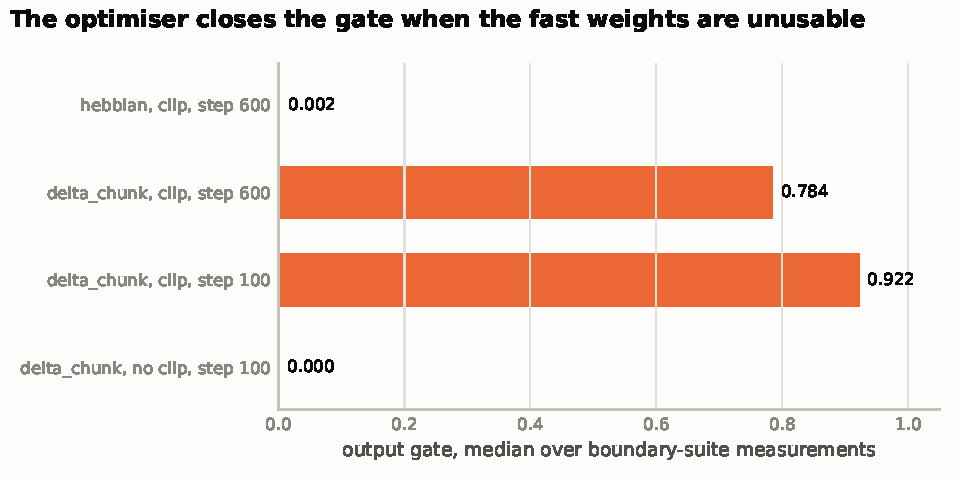
\includegraphics[width=0.8\linewidth]{figures/F12_gates.pdf}
  \caption{Median output gate under each configuration.}
  \label{fig-gates}
\end{figure}

\section{Summary}

The clip is what makes the fast weights usable at all, by reducing an unusably large state to a fixed and usable scale, and it does so precisely by discarding the magnitude that persistence would need. Within this architecture the carried state can be stable or keep its magnitude, but not both. With the clip in place, the direction it carries is uninformative even about the document that produced it. The cause of the null result is argued from the mechanism and supported by the probes, rather than shown by a single intervention. Chapter~\ref{ch-design} takes the opposite route and changes how the carry is read and trained, keeping the clip.

% ======================================================================
\chapter{A Carry That Works on Related Text}
\label{ch-design}

The previous chapters show that the carry, as first designed, contributes little even between slices of the same document, where the text it carries is directly relevant. Four features of the training setup explain why. The carried state was detached between slices, so only the parts of the model that read the carry were trained, never the parts that decide what to write. The carry was added into the same sum as the current slice's state and clipped together with it, so the current slice could drown it. The Hebbian state saturates the clip. And the Hebbian rule starts training with a loss spike during which the fast weights are unusable. This chapter redesigns the carry against these four points, for the Hebbian rule, which is cheaper to train, and tests the result with the same evaluation protocol.

\section{Design}

All changes are configuration options, and every other setting is identical to the original Hebbian run.

\paragraph{A separate carry path.} The carried state is read through its own term with its own clip, gate and scale,
\begin{equation}
  \mathrm{out} = W_0 z + g(h)\, \eta\, S_{\mathrm{in}} z + \alpha\, g_c(h)\, \eta\, \mathrm{clip}(S_{\mathrm{carried}})\, z ,
\end{equation}
where $S_{\mathrm{in}}$ is the state built inside the current slice, $g_c$ is a second gate and $\alpha$ is a learnable scalar initialised to zero. At initialisation the layer is therefore exactly the original Hebbian layer, and the carried term enters only if training finds it useful.

\paragraph{Training through the carry.} The carried state is kept in the autograd graph between the slices of a session, so the loss on a later slice also trains what an earlier slice wrote. To bound memory, the carry is detached after every second slice and at every optimiser step. Gradient checkpointing re-runs each layer's forward pass during the backward pass, and with the carry in the graph a layer can be re-run after its carry has moved on, which silently corrupts the gradient. The recompute is therefore given the carry the layer actually read, and a test confirms that gradients with and without checkpointing are identical, and that they differ by up to several hundred percent without this correction.

\paragraph{A nearly closed main gate at the start.} The main gate's bias is initialised at $-6$ instead of $-2$, so the in-document fast weights start at about 0.25 percent strength rather than 12 percent. This is close to where the original Hebbian model's gate ends after training (0.002).

\section{Two failed attempts}

The design above is the third attempt, and the first two explain its last two features. Their in-training evaluations are kept in the results folder.

The first attempt used the separate carry path without the zero-initialised scale and with the usual gate bias of $-2$. At step 100, carrying state between slices raised perplexity from 16.3 to 31.5, worse on every source. The reason is the size of a clipped state. The clip bounds the state at $\tau = 20$, which is 4 to 5 times the largest singular value of the pretrained down-projection (3.8 to 4.8 in layers 1, 13 and 27). A clipped state concentrated in few directions, as outer-product states tend to be, therefore adds about half the strength of $W_0$ along those directions even through a gate at 12 percent. The zero-initialised scale removes this.

The second attempt added the scale but kept the gate bias at $-2$. This time the in-document fast weights, not the carry, broke the model during early training. With them switched on, perplexity was 4703 at step 50 and 1024 at step 100, against 16.6 and 16.2 with them off, and the training loss opened at 17.5. The carry cannot be the cause, since its scale starts at zero and the failing regime resets the state at every slice, so the spike comes from the Hebbian fast weights within a slice. The model recovered by step 150, but the spike wasted most of a short run. Closing the gate at the start removes it. The second attempt also ran out of GPU memory near step 195, because training through the carry held every slice of a long document in memory, which the window of two slices fixes.

\section{Results}

With all four changes the training loss stays between 2.0 and 2.6 from step 10. The design was trained twice with the same configuration and seed, once to step 200 with full evaluations at steps 100 and 200, and once to step 600 with full evaluations at steps 400 and 600. From step 200 on, the boundary suite uses chains of 20 documents per source, so the cross-document measure rests on 100 documents instead of 24. Table~\ref{tab-design} and Figure~\ref{fig-design} compare the design with the original Hebbian model, and Figure~\ref{fig-design-curve} shows the carry gains across training.

\begin{table}[H]
  \centering
  \caption{The carry design against the original Hebbian model, gains in perplexity with the share of documents improved in brackets. A star marks a 95 percent interval that excludes zero. The cross-document measure rests on 24 documents for the original model and at step 100, and on 100 documents otherwise.}
  \label{tab-design}
  \small
  \begin{tabular}{lrrrrr}
    \toprule
    & Hebbian & \multicolumn{4}{c}{Carry design} \\
    \cmidrule(lr){2-2} \cmidrule(lr){3-6}
    Measure & step 600 & step 100 & step 200 & step 400 & step 600 \\
    \midrule
    Between slices, same document & $+0.002$ (0.54) & $+0.135$\sig\ (0.99) & $+0.099$\sig\ (0.92) & $+0.062$\sig\ (0.92) & $+0.097$\sig\ (0.97) \\
    Into a different document & $-0.004$ (0.38) & $+0.011$\sig\ (0.75) & $+0.010$\sig\ (0.64) & $-0.003$ (0.39) & $-0.020$\sig\ (0.29) \\
    Within a slice & $+0.034$\sig\ (0.89) & $+0.047$\sig\ (0.83) & $+0.018$\sig\ (0.74) & $+0.006$\sig\ (0.63) & $+0.025$\sig\ (0.76) \\
    Lead over matched LoRA & $+0.106$\sig\ (1.00) & n/a & $+0.215$\sig\ (0.98) & $+0.188$\sig\ (1.00) & $+0.234$\sig\ (1.00) \\
    \bottomrule
  \end{tabular}
\end{table}

\begin{figure}[H]
  \centering
  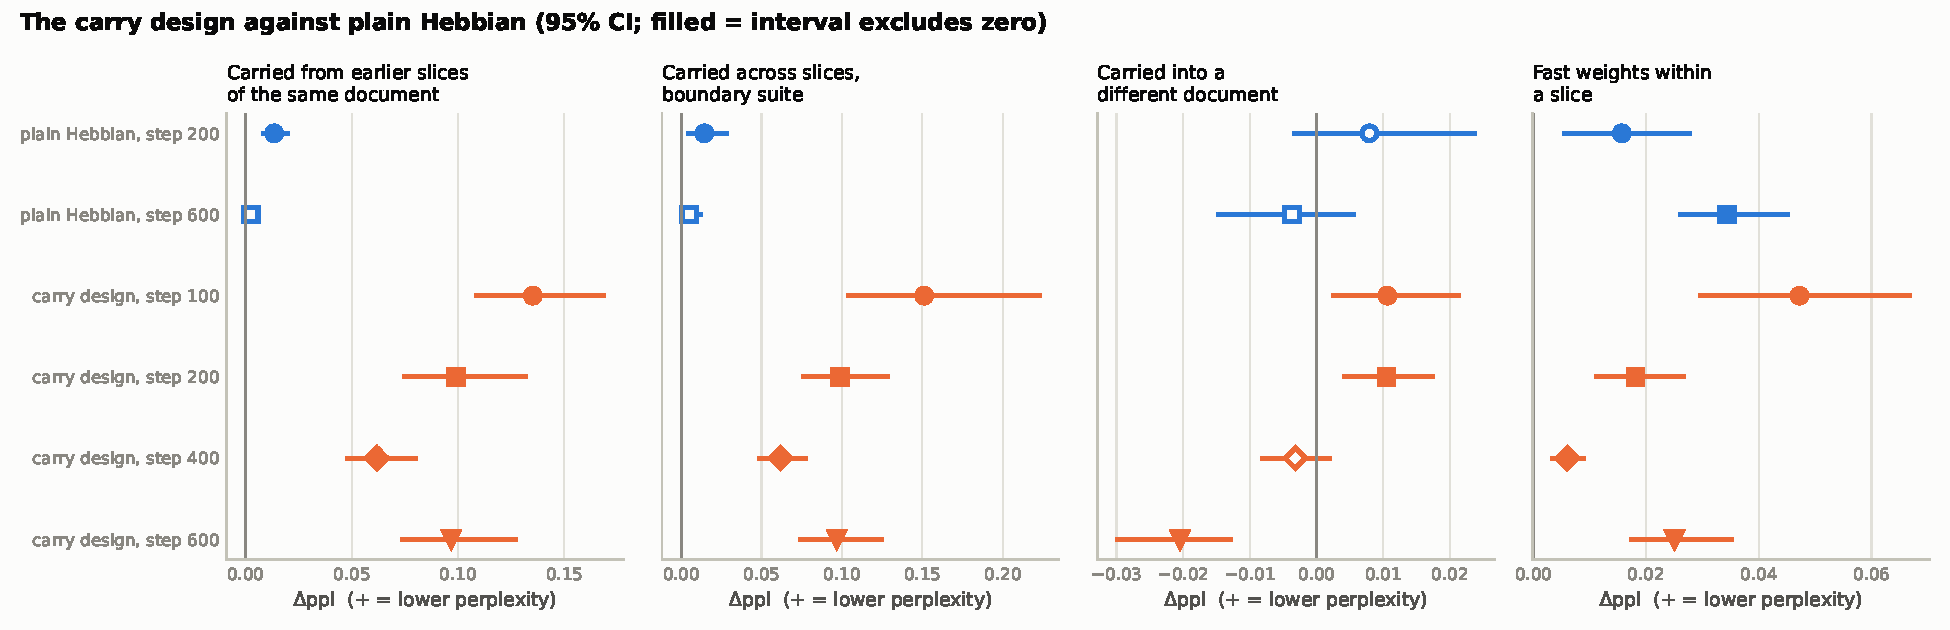
\includegraphics[width=\linewidth]{figures/F13_carry_design.pdf}
  \caption{The carry design against the original Hebbian model, with 95 percent bootstrap intervals. A filled marker means the interval excludes zero.}
  \label{fig-design}
\end{figure}

\begin{figure}[H]
  \centering
  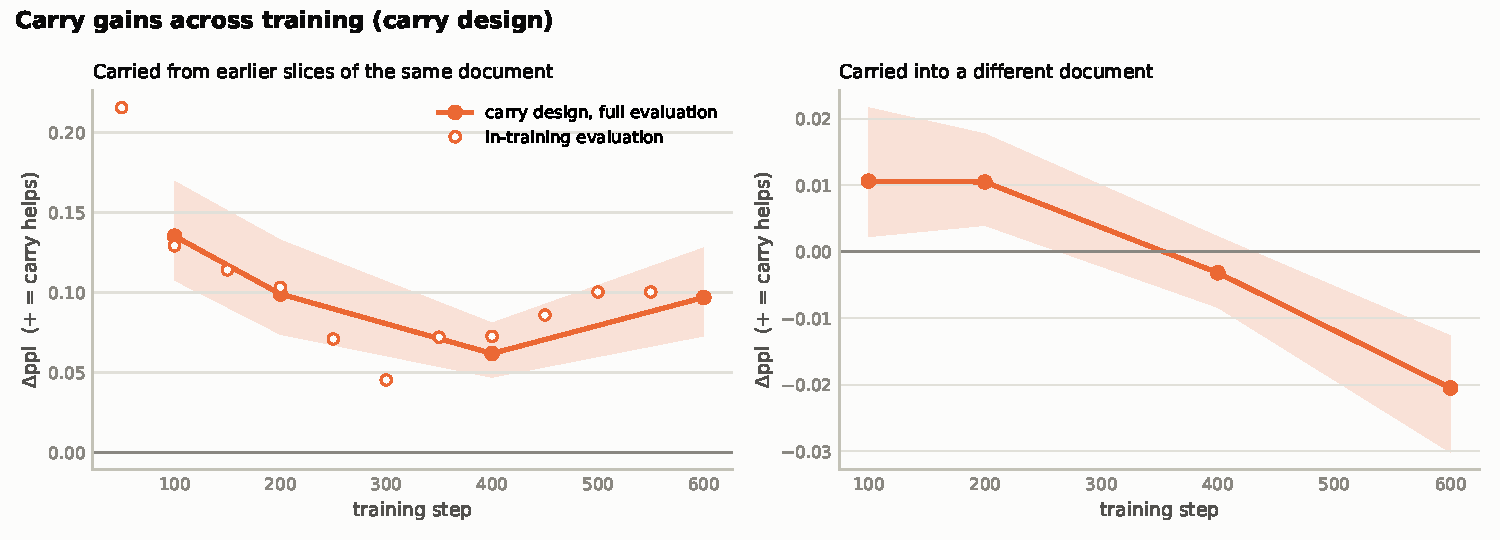
\includegraphics[width=\linewidth]{figures/F15_carry_design_curve.pdf}
  \caption{Carry gains of the carry design across training, with 95 percent bootstrap bands. Hollow markers are in-training evaluations on 30 documents without intervals. The cross-document point at step 100 rests on 24 documents and the others on 100.}
  \label{fig-design-curve}
\end{figure}

\paragraph{Carry within a document helps and survives full training.} Carrying state from earlier slices of the same document lowers perplexity by 0.135 at step 100, 0.099 at step 200, 0.062 at step 400 and 0.097 at step 600, every interval excluding zero, on 92 to 99 percent of documents. The original design's gain is 0.014 at step 200 and 0.002 at step 600. The in-training evaluations follow the same course, a dip around steps 250 to 400 and a recovery to about 0.10 by step 500, so the gain does not vanish as the slow weights train.

\paragraph{It helps from the second slice on and does not accumulate.} At step 600 the gain is between 0.099 and 0.121 at every slice from the second to the eighth, each interval excluding zero (Figure~\ref{fig-design-slice}). The in-training evaluations show the same flat profile at every step, with a late-minus-early trend between $-0.10$ and $+0.01$. The carry acts as a memory of the recent text of the document rather than one that keeps accumulating.

\begin{figure}[H]
  \centering
  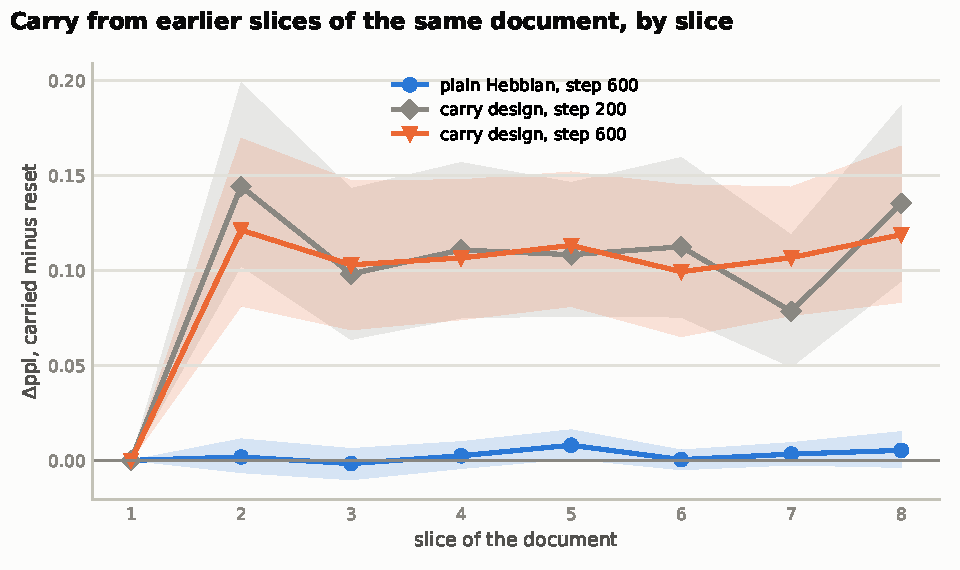
\includegraphics[width=0.8\linewidth]{figures/F14_carry_design_by_slice.pdf}
  \caption{Gain from carrying state from earlier slices of the same document, by slice, with 95 percent bootstrap bands.}
  \label{fig-design-slice}
\end{figure}

\paragraph{Across documents the carry turns from a small help into a small harm.} With 100 documents, carrying state into a different document of the same source lowers perplexity by 0.010 $[+0.004, +0.018]$ at step 200, mainly on C4 and Wikipedia. By step 400 the effect is gone ($-0.003$), and at step 600 the carried state makes perplexity worse, by 0.020 $[-0.030, -0.013]$, on 71 percent of documents, with a significant harm on four of the six sources. Training therefore makes the carry more specific to the text it was built from. It continues the same document as well as ever, while for an unrelated document it becomes interference.

\paragraph{The carry recovers about four percent of the preceding text.} The context suite compares the carry with placing the previous slice directly in attention, scoring the same tokens. At step 600 the previous slice in attention lowers perplexity by 2.770 (25.7 percent), the carried state by 0.110, so the carry recovers 4.0 percent $[3.3, 4.7]$ of that gain, and 3.9 percent $[3.1, 4.6]$ at step 200. The carried state is a much weaker channel than attention when the text is still available. Its size is fixed rather than small. It holds 44.0 million values, which in the 32-bit precision used here take about 176 MB, as much as the 16-bit attention cache of roughly 1500 tokens of Qwen3-0.6B (28 layers, 8 key-value heads of dimension 128). Its use is therefore where attention cannot reach, not as a cheaper substitute for it.

\paragraph{Overall, the design outperforms both original rules.} The main gate stays nearly closed (median 0.0007 at step 200), so the benefit flows through the carry path. The model leads the matched LoRA baseline by 0.234 perplexity at step 600 on every document, against 0.106 for the original Hebbian model and 0.203 for the delta rule at the same step.

\section{Which design change matters}

The design combines three changes, the separate carry path (A), training through the carry (B) and the nearly closed main gate at the start (C). Three further runs, each trained to step 200 with the same data and seed, remove ingredients in turn. The fourth combination, A and B without C, is the second failed attempt above, whose early instability made it unusable. Table~\ref{tab-ablation} and Figure~\ref{fig-ablation} compare them with the full design at step 200.

\begin{table}[H]
  \centering
  \caption{Ablation of the carry design at step 200, gains in perplexity with 95 percent intervals. Every interval excludes zero.}
  \label{tab-ablation}
  \small
  \begin{tabular}{lrrr}
    \toprule
    Variant & Between slices & Into a different document & Lead over matched LoRA \\
    \midrule
    Closed gate only (C) & $+0.008$ & $+0.003$ & $+0.130$ \\
    Carry path, no training through it (A and C) & $+0.023$ & $+0.011$ & $+0.172$ \\
    Training through it, no carry path (B and C) & $+0.035$ & $+0.014$ & $+0.163$ \\
    Full design (A, B and C) & $+0.099$ & $+0.010$ & $+0.215$ \\
    \bottomrule
  \end{tabular}
\end{table}

\begin{figure}[H]
  \centering
  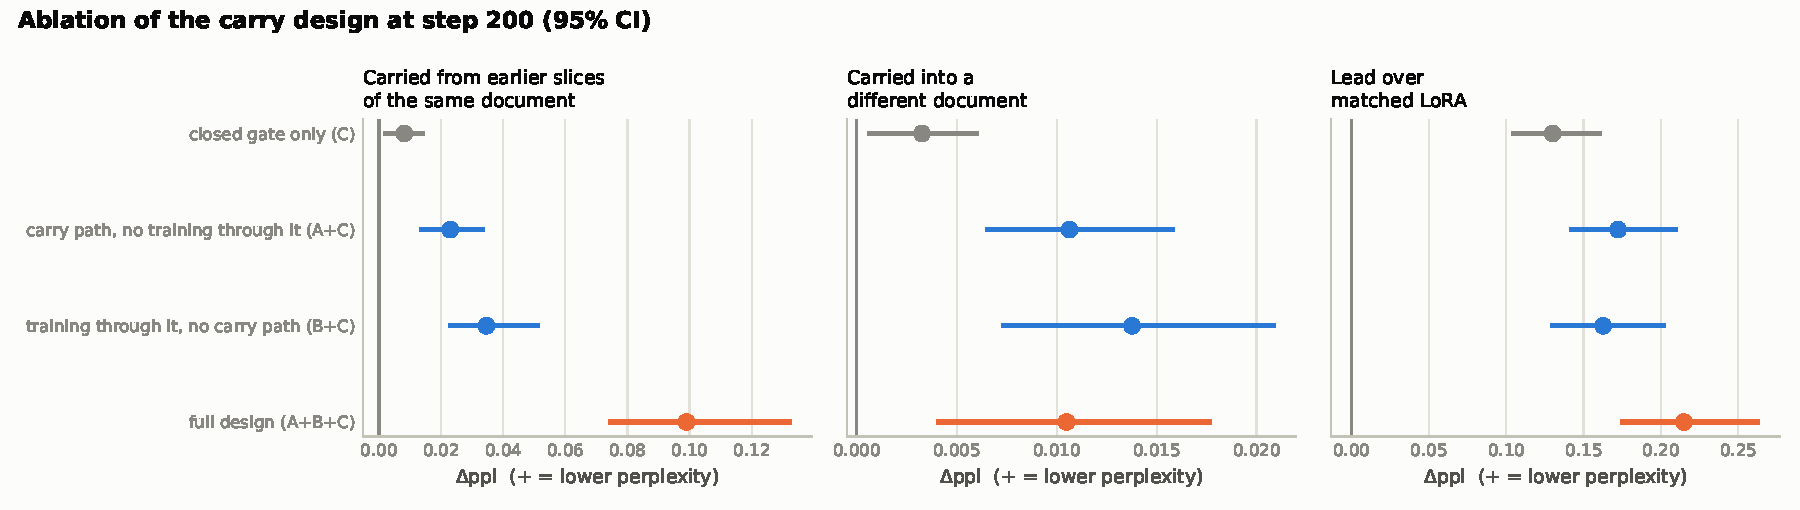
\includegraphics[width=\linewidth]{figures/F17_ablation.pdf}
  \caption{Ablation of the carry design at step 200, with 95 percent bootstrap intervals.}
  \label{fig-ablation}
\end{figure}

\paragraph{The closed gate does not explain the gain.} With the closed gate alone, the carry between slices gives 0.008, close to the original design's 0.014. Starting the gate nearly closed only removes the early instability.

\paragraph{The two carry changes work together.} The separate carry path alone raises the carry gain to 0.023, and training through the carry alone to 0.035. Together they give 0.099, more than twice the sum of their separate increments over the closed gate alone (0.015 and 0.027 against 0.091). The separate path lets a carried state reach the output without being drowned by the current slice, and training through the carry teaches the model what to write for a later slice to read, and each is of limited use without the other. The lead over the matched baseline follows the same order, from 0.130 with the closed gate alone to 0.215 with the full design.

\paragraph{Cross-document carry is small in every variant.} At step 200 every variant carries a small benefit into a different document, between 0.003 and 0.014, with overlapping intervals. The relatedness effects of the full design therefore come with training through the carry over the full 600 steps rather than from any one change at step 200.

\section{A relatedness gradient}

The comparison so far has two points, the same document and a different document of the same source. To test documents that are distinct but related, a further suite uses English Wikipedia, a source on which the carry works well (Table~\ref{tab-sources}). Two shards of the November 2023 English dump give 55{,}761 articles, of which 18{,}747 are long enough to serve as targets. For each of 200 target articles, chosen in a seeded order, the second block of 1024 tokens is scored after the carry is reset and after it is primed by a block of 1024 tokens from one of four texts, ordered by relatedness.
\begin{description}
  \item[Same document.] The target article's own first 1024 tokens.
  \item[Related article.] The article the target mentions most often by title, at least twice, matching whole multi-word titles only.
  \item[Random article.] An article that neither mentions the target nor is mentioned by it.
  \item[Other source.] A held-out document from one of the other five SlimPajama sources.
\end{description}
Every prime has the same length and every arm scores exactly the same target tokens, so only the relatedness of the prime varies. The same 200 cases, identical title for title, were measured on the carry design and on the original Hebbian model, both at step 600.

\begin{table}[H]
  \centering
  \caption{Gain from the carry by relatedness of the priming text, against a reset carry, on the same 200 Wikipedia targets at step 600. Shares of targets improved in brackets. A star marks a 95 percent interval that excludes zero.}
  \label{tab-related}
  \small
  \begin{tabular}{lrr}
    \toprule
    Carry built from & Original Hebbian & Carry design \\
    \midrule
    Same document & $-0.002$ (0.50) & $+0.103$\sig\ (0.89) \\
    Related article & $+0.004$ (0.59) & $+0.085$\sig\ (0.85) \\
    Random article & $+0.001$ (0.48) & $+0.051$\sig\ (0.70) \\
    Other source & $-0.013$\sig\ (0.39) & $-0.067$\sig\ (0.28) \\
    \midrule
    Same document against related & $-0.005$\sig & $+0.018$\sig \\
    Related against random & $+0.003$ & $+0.034$\sig \\
    Random against other source & $+0.013$\sig & $+0.117$\sig \\
    \bottomrule
  \end{tabular}
\end{table}

\begin{figure}[H]
  \centering
  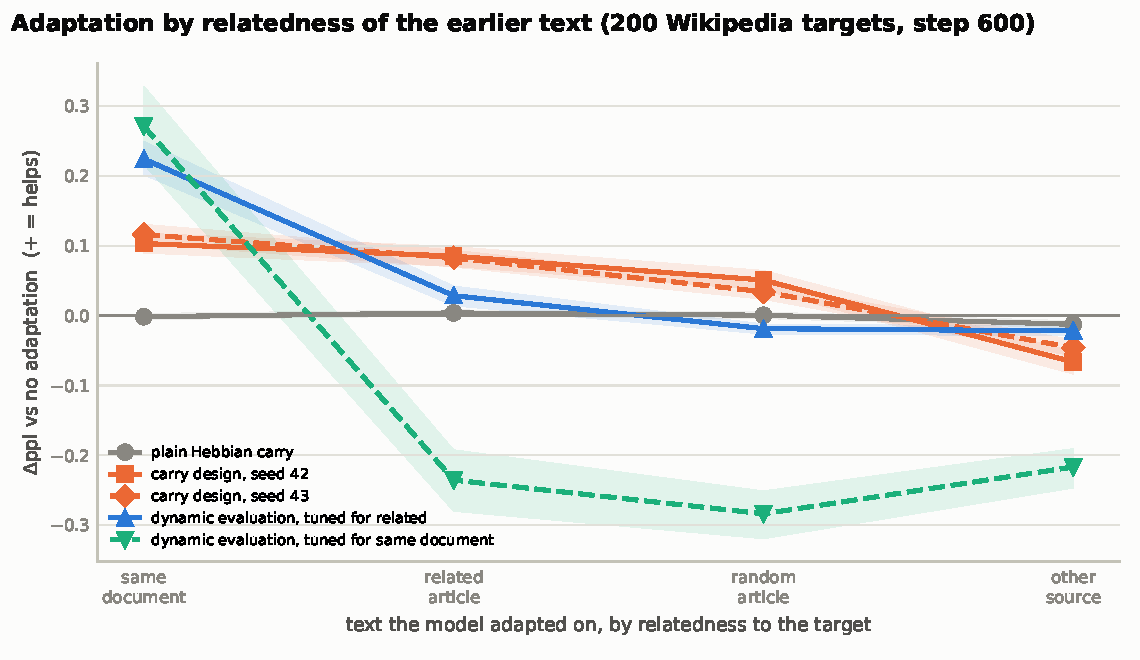
\includegraphics[width=0.8\linewidth]{figures/F16_relatedness.pdf}
  \caption{Gain from adapting on earlier text, by its relatedness to the target, on the same 200 Wikipedia targets at step 600, with 95 percent bootstrap bands. The carry design with two training seeds, the original Hebbian carry, and dynamic evaluation of the LoRA-only model tuned for the related arm and for the same-document arm (Section~\ref{sec-dyneval}).}
  \label{fig-related}
\end{figure}

\paragraph{The carry's effect falls steadily with relatedness.} For the carry design every step down the scale is significant (Table~\ref{tab-related}, Figure~\ref{fig-related}). A carry built from the same article lowers perplexity by 0.103, one built from an article the target mentions by 0.085, one built from an unrelated article by 0.051, and one built from a different source raises it by 0.067. The key contrast, a related article against an unrelated one, is $+0.034$ $[+0.024, +0.044]$, in favour of the related article on 70 percent of targets. A distinct but related document therefore helps clearly more than an unrelated one.

\paragraph{The gradient belongs to the redesign.} On the same cases the original Hebbian carry has no significant gain at any level, and only a small harm from other-source text. The graded pattern, its help and its harm, appear only with the redesigned carry.

\paragraph{Robustness.} Title matching also links articles to date pages, such as an article mentioning ``August 1''. Removing the 18 targets whose related prime is a date page leaves every estimate within 0.003 of the full result, including the related against random contrast ($+0.034$ $[+0.023, +0.045]$, 182 targets).

\paragraph{A random article still helps.} Unlike the cross-document result of the boundary suite, where a carried state from another document of the same source harmed perplexity at step 600, an unrelated Wikipedia article helps here. The setups differ in what is carried. Here the prime is the opening block of one Wikipedia article, a summary written in the same encyclopedic style as the target. The boundary suite instead carries the decayed state of several whole earlier documents of the same source, each read in eight slices, and pools six sources of which most are less uniform in style than Wikipedia. A plausible reading, not tested here, is that a single short block mainly transfers shared style, which helps, while a long accumulation of unrelated content mainly adds interference. The two results agree on the ordering, with the most related text helping most and text from another source harming.

\section{Comparison with dynamic evaluation}
\label{sec-dyneval}

Dynamic evaluation \citep{krause2018dynamic} is the established way to carry adaptation from one text to the next. The model takes gradient steps on the text it has just read and reads the next text with the adapted weights. As a baseline, the LoRA-only model at step 600 takes Adam steps on its 10.1 million LoRA parameters over each prime, reads the target, and has its weights restored exactly before the next case, with the update made on 32-bit copies so that small steps are not lost to 16-bit rounding. This is the sparse form of dynamic evaluation that \citet{krause2018dynamic} found to recover most of the full method's gain.

\paragraph{Tuning.} The step size and number of steps were chosen on 40 further Wikipedia cases, disjoint from the 200 reported, separately for two objectives, the gain on the same document and the gain from a related article. A first, coarser search showed plain gradient descent far below Adam at every step size it tried (at most 0.149 against 0.441), and Adam degrading sharply from a step size of $3 \times 10^{-4}$, so the final grid uses Adam with step sizes from $3 \times 10^{-6}$ to $10^{-4}$ and 3, 10 or 30 steps. For each objective the best settings lie on a ridge of roughly constant step size times number of steps, about $10^{-4}$ for the related arm and $3 \times 10^{-4}$ for the same document, and settings beyond the ridge diverge, so the grid brackets the optimum. Tuned for the same document the best setting is a step size of $3 \times 10^{-5}$ with 10 steps, and tuned for a related article it is $3 \times 10^{-5}$ with 3 steps. The reported cases are identical, title for title, to those of the carry.

\paragraph{Results.} Figure~\ref{fig-related} shows both baselines beside the carry, and Table~\ref{tab-dyneval} gives the paired difference between the carry and dynamic evaluation tuned for the related arm, case by case, as the difference in log-perplexity gain in percent.

\begin{table}[H]
  \centering
  \caption{The carry design against dynamic evaluation tuned for the related arm, on the same 200 Wikipedia targets at step 600. Each cell is the carry's gain minus dynamic evaluation's, in percent of log-perplexity, with a 95 percent bootstrap interval and the share of targets on which the carry gains more. Positive values favour the carry.}
  \label{tab-dyneval}
  \small
  \begin{tabular}{lrr}
    \toprule
    Adapted on & Carry seed 42 & Carry seed 43 \\
    \midrule
    Same document & $-0.67\%$ {\footnotesize [$-0.81$, $-0.55$]} (0.20) & $-0.60\%$ {\footnotesize [$-0.74$, $-0.47$]} (0.28) \\
    Related article & $+0.32\%$ {\footnotesize [$+0.21$, $+0.43$]} (0.72) & $+0.31\%$ {\footnotesize [$+0.22$, $+0.39$]} (0.70) \\
    Random article & $+0.39\%$ {\footnotesize [$+0.30$, $+0.47$]} (0.73) & $+0.29\%$ {\footnotesize [$+0.23$, $+0.36$]} (0.68) \\
    Other source & $-0.25\%$ {\footnotesize [$-0.35$, $-0.17$]} (0.41) & $-0.14\%$ {\footnotesize [$-0.21$, $-0.07$]} (0.42) \\
    \bottomrule
  \end{tabular}
\end{table}

\paragraph{The carry transfers more, dynamic evaluation fits more.} Dynamic evaluation tuned for a related article lowers perplexity by 0.224 on the same document, but only by 0.029 from a related article, and it slightly harms after an unrelated article ($-0.019$) or another source ($-0.022$). The carry gains less on the same document and clearly more from a related article (0.085) and from an unrelated article of the same source (0.051). Paired case by case, the carry's transfer to a related article exceeds dynamic evaluation's by 0.32 and 0.31 percent at the two seeds, and its transfer to an unrelated article by 0.39 and 0.29 percent, while dynamic evaluation is better on the document's own text by 0.6 to 0.7 percent and the carry is more harmful after text from another source. Gradient steps fit the specific text they were taken on, which pays off when the same text continues and transfers poorly to anything else, while the carry, trained to be read by a later slice, holds what transfers.

\paragraph{Tuned for the same document, dynamic evaluation overfits.} With the setting tuned for the same document, dynamic evaluation lowers perplexity on the document's own text by 0.271 but raises it by 0.236 after a related article and by 0.284 after an unrelated one. The setting that is best for the text just read is harmful for every other text.

\paragraph{Cost.} The carry is built during the ordinary forward pass and needs no backward pass. Dynamic evaluation tuned for related text needs three forward and backward passes over each prime, and tuned for the same document ten, and it must keep the adapted LoRA weights, 10.1 million values, against the carry's 44.0 million.

\section{The carry does not accumulate}

A memory that kept learning would help more each time it saw the same text. The repeat suite reads each of the 106 held-out SlimPajama documents ten times in a row with the carried state never reset, and compares later readings with earlier ones.

\begin{table}[H]
  \centering
  \caption{Reading the same document repeatedly with the carry never reset, at step 600, 106 documents, gains in perplexity with 95 percent intervals.}
  \label{tab-repeat}
  \small
  \begin{tabular}{lrr}
    \toprule
    Model & Second reading against first & Tenth against second \\
    \midrule
    Original Hebbian & $+0.001$ {\footnotesize [$-0.001$, $+0.002$]} & $+0.000$ {\footnotesize [$-0.001$, $+0.001$]} \\
    Carry design, seed 42 & $+0.006$\sig {\footnotesize [$+0.003$, $+0.009$]} & $+0.000$ {\footnotesize [$-0.001$, $+0.001$]} \\
    Carry design, seed 43 & $+0.008$\sig {\footnotesize [$+0.005$, $+0.012$]} & $-0.001$ {\footnotesize [$-0.002$, $+0.000$]} \\
    \bottomrule
  \end{tabular}
\end{table}

A second reading with the carried state helps slightly for the carry design, and every further reading adds nothing, although the carried state keeps growing, by a factor of about 3.4 from the second reading to the tenth (Table~\ref{tab-repeat}). The gain here is small because each document is read whole as one item, so the fast weights inside the document already capture most of what a reading offers. Together with the flat profile across the slices of a document, this shows that the carry passes on what the most recent text offers and does not build up knowledge with further exposure. It is a memory of recent related text, not a mechanism of continual improvement.

\section{Carry helps on related text and harms on unrelated text}

The same mechanism, in the same model, helps on the continuation of the same document throughout training, transfers to a distinct but related document more than dynamic evaluation does, and harms when the next text comes from another source. The relatedness suite turns this into a graded result. The carry's benefit falls with relatedness, from the same document to a related article to an unrelated article of the same source, and it becomes harm for text from another source. A trained, gated fast-weight carry is therefore a reliable memory of related text, worth up to about one percent in perplexity, and interference for unrelated text. This agrees with the swap result of Chapter~\ref{ch-q1}, where for the original Hebbian model a state primed on a different source made perplexity worse. It also implies that a deployed carry needs a way to decide when to apply it, such as resetting on a change of topic.

\section{Replication with a second seed}

The full design was trained again to step 600 with a second seed, which changes the training data order, the sampling of training documents and the dropout, and was evaluated on the same held-out documents. The relatedness suite selects its cases with its own fixed seed, so both runs were measured on the same 200 Wikipedia cases, identical title for title. Table~\ref{tab-seeds} compares the two seeds.

\begin{table}[H]
  \centering
  \caption{The carry design with two training seeds, gains in perplexity at step 600. A star marks a 95 percent interval that excludes zero.}
  \label{tab-seeds}
  \small
  \begin{tabular}{lrr}
    \toprule
    Measure & Seed 42 & Seed 43 \\
    \midrule
    Between slices, same document & $+0.097$\sig & $+0.092$\sig \\
    Into a different document (100 documents) & $-0.020$\sig & $-0.031$\sig \\
    Within a slice & $+0.025$\sig & $+0.014$\sig \\
    Lead over matched LoRA & $+0.234$\sig & $+0.214$\sig \\
    Carry share of the previous slice in context & 4.0\% & 3.8\% \\
    \midrule
    Relatedness, same document & $+0.103$\sig & $+0.116$\sig \\
    Relatedness, related article & $+0.085$\sig & $+0.083$\sig \\
    Relatedness, random article & $+0.051$\sig & $+0.034$\sig \\
    Relatedness, other source & $-0.067$\sig & $-0.046$\sig \\
    Related against random & $+0.034$\sig & $+0.049$\sig \\
    \bottomrule
  \end{tabular}
\end{table}

Every result replicates in sign and significance, and most in size. The carry between slices of the same document is 0.097 and 0.092, the lead over the matched baseline 0.234 and 0.214, and the carry recovers 4.0 and 3.8 percent of the gain from the previous slice in attention. The relatedness gradient is monotone and significant at every step in both seeds, and its key contrast, a related article against a random one, is in fact larger with the second seed (0.049 against 0.034). The cross-document harm is stronger with the second seed ($-0.031$, worse on 84 percent of documents), and at this seed significant on all six sources, against four with the first. At step 400 the two seeds also agree, with carry between slices of 0.062 in both and a lead over the baseline of 0.188 and 0.180.

\section{What this chapter does not establish}

The ablation is measured at step 200 only, while the relatedness and cross-document results come from step 600. The main results replicate across two seeds, but the ablation and the failed attempts rest on one, and the delta rule was not redesigned. Relatedness is measured on Wikipedia only, and through title mentions, which is a coarse proxy. The context comparison gives the carry one previous slice of text, while the carry itself holds a decayed summary of all earlier slices. Dynamic evaluation was run in its sparse form on LoRA weights, the form that matches the carry's parameter budget, not on all weights.

% ======================================================================
\chapter{Discussion}
\label{ch-discussion}

\section{Relation to the update-rule literature}

The delta rule's advantage over the Hebbian rule matches the literature closely. \citet{schlag2021linear} and \citet{yang2024deltanet} predict that an additive store saturates through interference and cannot overwrite stale associations, and \citet{wang2026learning} find an error-correcting write better than In-Place TTT's additive one. Here the delta rule gives a within-document gain up to nine times larger, and only the Hebbian model collapses without the clip, which matches the observation of \citet{schlag2021linear} that the additive rule is unstable without normalisation. The gate closing on the Hebbian model echoes \citet{yang2024gla}, where an ungated additive accumulator trains poorly, and the finding of \citet{mao2022finetuning} that whether error correction helps depends on stabilisation.

\section{Relation to persistence and continual learning}

The null result for cross-document carry is consistent with the stability-plasticity dilemma \citep{french1999catastrophic}. The read-time clip buys stability by removing plasticity in the one quantity, the state's magnitude, that a carry needs to accumulate evidence. Successful persistence mechanisms in the literature avoid this in different ways. Transformer-XL and the Recurrent Memory Transformer carry activations or memory tokens within one stream and train through them \citep{dai2019transformerxl,bulatov2022rmt}, dynamic evaluation anchors updates to the trained weights with a decay \citep{krause2018dynamic}, and gated and selective state updates let a model choose what to keep \citep{gu2024mamba,yang2025gated}. The carry studied here has a fixed decay and no selectivity, and it receives no training signal across documents, since training sessions never cross a document boundary and backpropagation stops at each item.

\section{Related versus unrelated text}

The redesigned carry separates two questions that the original design left entangled. Whether a carried fast weight can hold useful information is answered yes, since it helps on the continuation of the same document once it is read through its own path and trained through. Whether it transfers beyond that document is answered by the relatedness gradient. It transfers to a related article, more than dynamic evaluation does, less to an unrelated article of the same source, and it harms after text from another source. The contrast with dynamic evaluation suggests why. Gradient steps fit the text they were taken on, while a carry that was trained to be read by a later slice learns to hold what a later text can use. The update-rule and continual-learning literature anticipates both halves. Gated and selective memories, which decide what to keep \citep{gu2024mamba,yang2025gated}, and persistence mechanisms trained through the boundary \citep{dai2019transformerxl,bulatov2022rmt}, are the ingredients the redesign adds, and the stability-plasticity view \citep{french1999catastrophic} predicts that a memory tuned to recent context will not transfer to unrelated input.

\section{Implications}

For practitioners, the results suggest that a carried fast weight is worth keeping across documents only when the next document is related, and that it should be reset when the topic or source changes, while within a document attention remains far stronger. For research on session-persistent test-time learning, they suggest that a carried state needs a bound that is part of its design rather than imposed at read time, for example a normalised or gated memory that stores its magnitude in a usable range, and a training signal that spans document boundaries.

% ======================================================================
\chapter{Limitations and Future Work}
\label{ch-limits}

\paragraph{Capacity confound.} The TTT models train about 6.7 times as many parameters as the control. Most of their lead over the control is this extra capacity, and a control with matched parameter count, such as the same architecture trained with fast-weight updates disabled, would separate the two cleanly. It was not run for budget reasons. The within-document gain is the measure that isolates the mechanism.

\paragraph{Carry trained within documents only.} Every training session is one document, so the models learn to use a carried state between slices of a document but are never trained with a state carried from a different document. The cross-document result therefore measures whether a within-document carry transfers across documents, not what a model trained on multi-document sessions would learn. The clip analysis in Chapter~\ref{ch-why} applies to both cases, since the clip saturates on every measurement regardless of how the state was built.

\paragraph{Scale.} One model of 0.6 billion parameters is studied, against the 0.6 to 4 billion range planned in the proposal, with one seed per configuration except the carry design, which has two, and at most 600 of 1050 optimiser steps. The persistence result is stable across 200, 400 and 600 steps, which argues against undertraining within this budget, but larger models and longer training are untested.

\paragraph{Evaluation set.} The held-out set has 106 documents, with only 6 from Book. Per-source cross-document estimates rest on four documents each.

\paragraph{No-clip probes.} The runs without the clip are short, 100 to 200 steps, and single-seed. They show that removing the clip does not rescue persistence early in training, not what a long unclipped run would converge to.

\paragraph{Carry design.} The redesigned carry of Chapter~\ref{ch-design} is replicated with two seeds, which is enough to show its results are not a fluke but not to report a spread, its ablation stops at step 200 with one seed, and it exists for the Hebbian rule only. Its relatedness gradient is measured on Wikipedia only, with relatedness defined by title mentions, and the comparison with dynamic evaluation uses its sparse form on LoRA weights.

\paragraph{Perplexity only.} All evidence is perplexity-based. The RULER probes planned in the proposal were dropped once the carried effect measured zero, and no behavioural test of retained information was attempted, consistent with the proposal's scope.

\paragraph{Future work.} For the carry design, the most direct extensions are further seeds to report a spread, the relatedness gradient on other domains and with finer measures of relatedness, a mechanism that decides when to apply the carry, and the same design for the delta rule. More broadly, the extensions are a parameter-matched control, dynamic evaluation on all weights, a carried state with a designed bound such as a normalised or gated memory, training through document boundaries so that the carry receives a learning signal, and replication at larger scale with several seeds.

% ======================================================================
\chapter{Conclusion}
\label{ch-conclusion}

This thesis asked whether the fast weights that test-time training builds while reading one document can be carried into the next. They can, if the carry is designed and trained for it, and what they carry is specific. A trained, gated carry transfers to related documents and hurts unrelated ones. Its benefit falls steadily from a related article to an unrelated one and turns to harm for text from another source, it transfers more than dynamic evaluation tuned for the same purpose while needing only forward passes, and it holds across two training seeds. It is a memory of recent related text and not of everything read, since repeated reading adds nothing beyond the first, and next to attention on the preceding text it recovers only about four percent of the gain, so its place is where attention cannot reach.

Reaching this design required understanding why the naive carry fails. The norm clip that keeps the fast weights stable is saturated on every measurement, so a carried state reaches the output only as a direction, and removing the clip makes the model either collapse or switch the fast weights off. Giving the carry its own zero-initialised path and training it through the boundary between slices, two changes that only work together, turns it from no help into the strongest model in the study. Along the way the attribution shows that most of a TTT model's lead over a matched baseline is extra trainable capacity, and that within a document the delta rule adapts several times more than the Hebbian rule. The open questions are whether the gradient holds beyond Wikipedia and at larger scale, and how a model should decide when to apply its carry, since applying it to unrelated text does harm.

\bibliographystyle{plainnat}
\bibliography{references}

\appendix

\chapter{Hyperparameters}
\label{app-hparams}

\begin{table}[H]
  \centering
  \small
  \caption{Settings shared by all runs unless marked as TTT only.}
  \begin{tabular}{ll}
    \toprule
    Setting & Value \\
    \midrule
    Base model & Qwen3-0.6B \\
    TTT layers (TTT only) & 1, 3, 5, up to 27 (14 layers) \\
    Chunk size $C$ (TTT only) & 50 \\
    Fast-weight step $\eta$ (TTT only) & 2 \\
    Target convolution kernel (TTT only) & 8, causal, depthwise \\
    Output gate bias at initialisation (TTT only) & $-2$ \\
    Read-time clip $\tau$ (TTT only) & 20 \\
    Carried-state decay $\lambda$ (TTT only) & 0.9 \\
    Truncated backpropagation window, delta rule (TTT only) & 5 chunks \\
    LoRA rank, $\alpha$, dropout & 16, 32, 0.05 \\
    Learning rate, LoRA & $1 \times 10^{-5}$ \\
    Learning rate, TTT down-projection (TTT only) & $3 \times 10^{-5}$ \\
    Learning rate, new TTT modules (TTT only) & $6 \times 10^{-2}$ \\
    Weight decay, full parameters and LoRA & 0.1 and 0 \\
    Gradient clip & 10 \\
    Gradient accumulation & 16 \\
    Warmup & 2\% of steps, at least 10 \\
    Schedule & cosine over 1050 steps \\
    Training documents & 4000, 2048 to 16384 tokens \\
    Session strategy & one document, 2 to 6 slices of at least 1000 tokens \\
    Seed & 42 \\
    Bootstrap resamples & 1000 \\
    \midrule
    Carry design (Chapter~\ref{ch-design}) & separate carry path and gate, zero-initialised scale \\
    Carry design, training through the carry & window of 2 slices, detached at each optimiser step \\
    Carry design, main gate bias at initialisation & $-6$ \\
    \bottomrule
  \end{tabular}
\end{table}

\chapter{Full Results}
\label{app-full}

\begin{table}[H]
  \centering
  \caption{All pooled gaps with 95 percent bootstrap intervals and win rates.}
  \label{tab-full}
  \scriptsize
  \begin{tabular}{llrrr}
    \toprule
    Model and step & Measure & Gap & 95\% interval & Win rate \\
    \midrule
    LoRA-only 200 & training & $+1.610$ & [$+1.293$, $+2.013$] & 1.00 \\
    Hebbian 200 & training & $+1.653$ & [$+1.335$, $+2.057$] & 1.00 \\
    Delta 200 & training & $+1.670$ & [$+1.349$, $+2.074$] & 1.00 \\
    LoRA-only 400 & training & $+1.784$ & [$+1.440$, $+2.222$] & 1.00 \\
    Hebbian 400 & training & $+1.852$ & [$+1.499$, $+2.300$] & 1.00 \\
    Delta 400 & training & $+1.909$ & [$+1.542$, $+2.364$] & 1.00 \\
    LoRA-only 600 & training & $+1.859$ & [$+1.503$, $+2.310$] & 1.00 \\
    Hebbian 600 & training & $+1.928$ & [$+1.561$, $+2.392$] & 1.00 \\
    Delta 600 & training & $+1.992$ & [$+1.613$, $+2.465$] & 1.00 \\
    \midrule
    Hebbian 200 & within & $+0.016$ & [$+0.005$, $+0.028$] & 0.72 \\
    Delta 200 & within & $+0.144$ & [$+0.117$, $+0.179$] & 1.00 \\
    Hebbian 400 & within & $+0.014$ & [$+0.009$, $+0.020$] & 0.79 \\
    Delta 400 & within & $+0.059$ & [$+0.047$, $+0.073$] & 0.99 \\
    Hebbian 600 & within & $+0.034$ & [$+0.026$, $+0.045$] & 0.89 \\
    Delta 600 & within & $+0.058$ & [$+0.046$, $+0.073$] & 0.96 \\
    \midrule
    Hebbian 200 & between slices & $+0.014$ & [$+0.008$, $+0.021$] & 0.70 \\
    Delta 200 & between slices & $+0.027$ & [$+0.019$, $+0.037$] & 0.83 \\
    Hebbian 400 & between slices & $-0.002$ & [$-0.005$, $+0.001$] & 0.46 \\
    Delta 400 & between slices & $+0.007$ & [$+0.003$, $+0.012$] & 0.65 \\
    Hebbian 600 & between slices & $+0.002$ & [$-0.000$, $+0.006$] & 0.54 \\
    Delta 600 & between slices & $+0.012$ & [$+0.008$, $+0.018$] & 0.74 \\
    \midrule
    Hebbian 200 & matched & $+0.073$ & [$+0.057$, $+0.094$] & 0.91 \\
    Delta 200 & matched & $+0.232$ & [$+0.190$, $+0.280$] & 1.00 \\
    Hebbian 400 & matched & $+0.080$ & [$+0.066$, $+0.098$] & 0.99 \\
    Delta 400 & matched & $+0.191$ & [$+0.156$, $+0.231$] & 0.99 \\
    Hebbian 600 & matched & $+0.106$ & [$+0.086$, $+0.130$] & 1.00 \\
    Delta 600 & matched & $+0.203$ & [$+0.165$, $+0.249$] & 1.00 \\
    \midrule
    Hebbian 200 & cross-document & $+0.008$ & [$-0.004$, $+0.024$] & 0.50 \\
    Delta 200 & cross-document & $+0.003$ & [$-0.006$, $+0.012$] & 0.58 \\
    Hebbian 400 & cross-document & $-0.003$ & [$-0.010$, $+0.002$] & 0.50 \\
    Delta 400 & cross-document & $+0.006$ & [$-0.000$, $+0.013$] & 0.67 \\
    Hebbian 600 & cross-document & $-0.004$ & [$-0.015$, $+0.006$] & 0.38 \\
    Delta 600 & cross-document & $-0.002$ & [$-0.006$, $+0.002$] & 0.38 \\
    \midrule
    Hebbian 200 & cross-slice & $+0.014$ & [$+0.003$, $+0.030$] & 0.83 \\
    Delta 200 & cross-slice & $+0.027$ & [$+0.013$, $+0.048$] & 0.77 \\
    Hebbian 400 & cross-slice & $+0.004$ & [$-0.002$, $+0.011$] & 0.60 \\
    Delta 400 & cross-slice & $+0.002$ & [$-0.004$, $+0.008$] & 0.60 \\
    Hebbian 600 & cross-slice & $+0.005$ & [$-0.001$, $+0.014$] & 0.60 \\
    Delta 600 & cross-slice & $+0.015$ & [$+0.005$, $+0.029$] & 0.73 \\
    \bottomrule
  \end{tabular}
\end{table}

\chapter{Reproducibility and Provenance}
\label{app-repro}

Every table and figure is regenerated from the stored evaluation bundles, without a GPU, by two commands, \texttt{python -m ttt.experiments.paper\_analysis\_v1} and \texttt{python -m ttt.experiments.thesis\_figures\_v1}. Each bundle stores its raw per-document rows and a manifest with the exact configuration and code version of the checkpoint it measured. \todo{code repository link and final commit hash}

Two provenance notes apply. Checkpoints of the Hebbian run after step 650 on one of the two storage volumes come from an earlier run with different settings and were excluded. The delta-rule run and the no-clip probes were evaluated from a second cloud workspace, whose storage volume uses some of the same run names for different runs. The bundle manifests record which checkpoint each result came from.

\end{document}
